\documentclass[10pt,a4paper]{report}
\usepackage{pdflscape} %Landscape format
\usepackage[T1]{fontenc}
\usepackage{graphicx}
\usepackage{subcaption}
\usepackage[ddmmyyyy]{datetime}
\usepackage{adjustbox}
\graphicspath{ {./images/} }
\usepackage{url}
%\usepackage{natbib}
\renewcommand{\bibname}{Kaynakça}
\renewcommand\thesection{\arabic{section}}
\renewcommand{\thesubfigure}{\thefigure\alph{subfigure}} % Alt şekil etiketini şekil 6b gibi ayarlar
\renewcommand{\figurename}{Şekil}
\DeclareUnicodeCharacter{202F}{\nobreakspace}



\title{Kalabalık Sayımı/Tespiti}

\author{Baki Dinç}
\begin{document}
	\textbf{KÜTAHYA SAĞLIK BİLİMLERİ ÜNİVERSİTESİ}\centering
	\begin{figure}[!h]
		\centering
		
\includegraphics[width=170px, height=170px]{logomuh}
		\maketitle
	\end{figure}
	
		\newpage
		
			\raggedright\section*{1.Giriş}
		Teknolojinin gelişimi, özellikle yapay zeka ve derin öğrenme alanındaki ilerlemeler, günlük yaşantımızdaki birçok alanda çeşitli çözümler sunmaktadır. Bu kapsamda, "Kalabalık Sayımı/Tespiti" adlı Projem, bir alışveriş merkezindeki kalabalığın veya merkezi bir caddede bulunan insanların (kalabalığın) sayılması üzerine odaklanmaktadır.\newline
		
		
		
		Bu proje ortak bir amacı, kalabalık alanlarda bulunan insan sayısını doğru ve etkili bir şekilde tespit ederek, çeşitli alanlarda güvenlik, operasyonel verimlilik, pazarlama stratejileri, salgın kontrolü ve müşteri deneyimi gibi çeşitli konularda kullanılabilecek veriler üretmektir.\newline
		

	
	
	
	\vspace{1cm}
	
		\textbf{Kalabalık Nedir ?}
	\raggedright	Kalabalık, bir alanda yoğun bir şekilde bulunan insan veya nesnelerin topluluğunu ifade eder. Anlam itibariyle genellikle bir insan grubunu tanımlamak için kullanılır, ancak aynı zamanda nesnelerin yoğun bir şekilde bulunduğu durumları da ifade edebilir.
	
	Örneğin, bir alışveriş merkezi, bir sokak, bir konser veya bir etkinlik alanı kalabalık olarak adlandırılabilir. Kalabalıklar genellikle insanların etkileşimde bulunduğu ve hareket ettiği yerlerdir.\newline 
	
	\textbf{Kalabalık çökmesi nedir ?}
	\raggedright Kalabalık çökmesi, bir bölgede çok yoğun bir kalabalık olduğunda ( > 5 kişi/m2), insanların vücudu birbirine temas halinde olup, birbirine itiş kuvveti uyguladığında ortaya çıkabiliyor. Bu kişilerden birinin düşmesi sonucunda, kişinin etrafındakilere uyguladığı itiş kuvveti kayboluyor ve çevresindekiler de adeta bir girdabın içine çekmesi misali düşen kişinin üzerine düşmeye başlıyor. Ve bu durum kitlede domino taşı benzeri etkiye yol açarak daha büyük bir girdapla sonuçlanıyor. Bu süreç, kalabalıktaki insanların birbirine temasıyla oluşan basınç rahatlayana kadar devam ediyor. Tabi bu girdapta altta kalanlar eziliyor, yaralanmalar ve asfiksi meydana geliyor. 2015’te Mekke’de Hac faaliyetinde 2000’den fazla kişinin ölümüyle sonuçlanan Mina İzdihamı buna örnek verilebilir\newline
	
	Teknolojinin gelişimi, özellikle yapay zeka ve derin öğrenme alanındaki ilerlemeler, günlük yaşantımızdaki birçok alanda çeşitli çözümler sunmaktadır. Bu kapsamda, "Kalabalık Sayımı/Tespiti" adlı Projem, bir alışveriş merkezindeki kalabalığın veya merkezi bir caddede bulunan insanların (kalabalığın) sayılması üzerine odaklanmaktadır.\newline
	
	
	
	Bu proje ortak bir amacı, kalabalık alanlarda bulunan insan sayısını doğru ve etkili bir şekilde tespit ederek, çeşitli alanlarda güvenlik, operasyonel verimlilik, pazarlama stratejileri, salgın kontrolü ve müşteri deneyimi gibi çeşitli konularda kullanılabilecek veriler üretmektir.\newline
	
	\clearpage
	
	Proje, bir gözetleme kamerası tarafından kaydedilen görüntüler üzerinde derin öğrenme tekniklerini kullanarak kalabalığı saymayı amaçlamaktadır.
	Bu projenin temel amaçlardan biri kalabalık ortamlarda kişi sayısını tahmin edip kalabalık ortamlarda alınabilecek tedbirlere ve kalabalığı yönlendirmeye veya korumaya yönelik tedbirler almayı amaçlamaktadır.\newline
	
	
	
	
	\section*{2 Tensorflow Nedir ? }
	
	TensorFlow temelde, makine öğrenimi uygulamaları ve sinir ağları geliştirmeye yönelik Python dostu bir açık kaynaklı kütüphanedir.
	
	Google Brain ekibi tarafından oluşturulan ve ilk kez 2015 yılında kamuoyuna sunulan TensorFlow, sayısal hesaplama ve büyük ölçekli makine öğrenimi için açık kaynaklı bir kütüphanedir. TensorFlow, bir dizi makine öğrenimi ve derin öğrenme modeli ve algoritmasını bir araya getirir ve bunları yaygın programlama metaforları aracılığıyla kullanışlı hale getirir. TensorFlow diğer birçok dil için kütüphaneler sağlar, ancak genellikle Python ön plandadır \cite{yegulalp2024}.
	
	\subsection*{2.1 Tensör nedir ?}
	
	Tensorflow'un adı doğrudan çekirdek çerçevesinden türetilmiştir: Tensor. Tensorflow'da tüm hesaplamalar tensörleri içerir. Tensör, tüm veri türlerini temsil eden n boyutlu bir vektör veya matristir. Bir tensördeki tüm değerler, bilinen (veya kısmen bilinen) bir şekle sahip aynı veri tipini içerir. Verinin şekli matrisin veya dizinin boyutluluğudur.
	
	Bir tensör, giriş verilerinden veya bir hesaplamanın sonucundan kaynaklanabilir. TensorFlow'da tüm operaişlemler bir grafik içerisinde gerçekleştirilir\cite{johnson2023}.\newline
	
	\begin{figure}[!h]
		\centering
		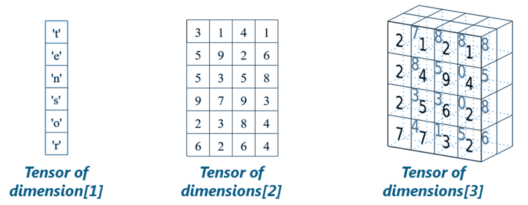
\includegraphics[width=\textwidth]{Tensor}
		\caption{ Tensor Matrisleri \cite{devhunter2018}}
		\label{Tensor}
	\end{figure}
	\clearpage
	
		\section*{3 Keras Nedir ? }
	Keras, Python'da yazılmış ve derin öğrenme için üst düzey bir kütüphane olarak inşa edilmiştir. Theano ve TensorFlow gibi alt yapıları kullanarak, çeşitli derin öğrenme modellerini oluşturmak için temiz ve kullanışlı bir arayüz sunar. Keras, sinir ağlarının geliştirilmesi ve test edilmesi için en yaygın kullanılan üst düzey sinir ağları API'lerinden biri haline gelmiştir.\newline
	
	Keras, kolay ve hızlı yöntemlerle model oluşturulmasına imkân sağlamaktadır. Bu özelliği ile yeni başlayanlar için modellerde, neler değiştirildiğinde nasıl bir etki yaratacağı deneme-yanılma yolu ile öğrenilmektedir.
	Modelleri merkezi işlem birimi (CPU) ve grafik işlemlerini yürüten işlemcileri (GPU) kullanarak sorunsuz biçimde çalıştırmaktadır. Bu şekilde istenildiği zaman işlemlerin GPU’da yapılarak zaman kazanılmasına destek olmaktadır.
	Bilgisayarlı görme modelleri olan evrişimsel sinir ağları CNN (Convolutional Neural Network) ve yinelemeli sinir ağlarını RNN (Recurrent Neural Network) desteklemektedir.
	İçerisinde kütüphane ile ilgili çok fazla kaynağın olması, oluşan ya da oluşabilecek sorunların yanıtına hızlı erişim imkânı sunmaktadır.
	
	\begin{figure}[!h]
		\centering
		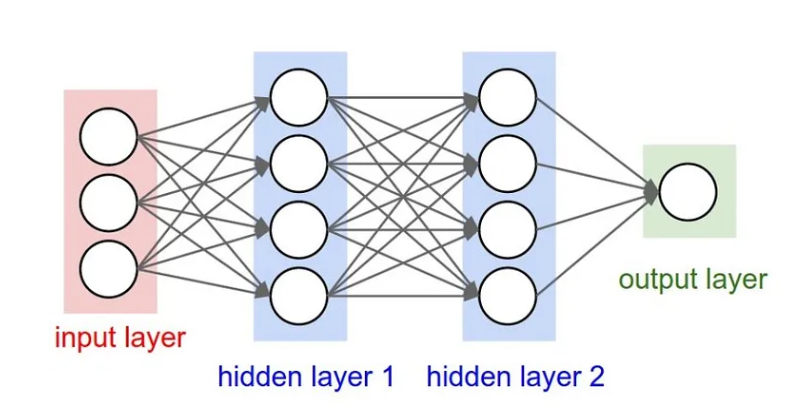
\includegraphics[width=\textwidth]{keras}
		\caption{ Keras \cite{allibhai}}
		\label{Keras}
	\end{figure}
	\clearpage
	İncelenen çalışma, CLIP (Contrastive Language-Image Pretraining) modelinin ve Geliştirilmiş Blok Bazlı Sınıflandırma (EBC) çerçevesinin kalabalık sayımı üzerindeki etkilerini Üzerine yoğunlaşmaktadır. Mevcut sınıflandırma tabanlı kalabalık sayımı yöntemlerinin karşılaştığı zorlukları ele alarak, CLIP ve EBC'nin birlikte kullanımının potansiyelini ortaya koyuyoruz. EBC, tam sayılı aralıklara dayanarak güçlü karar sınırlarının öğrenilmesini kolaylaştırırken, CLIP ise dil ve görüntü özelliklerini bir araya getirerek sayma görevine daha etkin bir şekilde yaklaşmayı sağlar. Bu çalışma, CLIP ve EBC'nin birlikte kullanımının, mevcut kalabalık sayımı yöntemlerine kıyasla alınan sonuçlardan yola çıkarak daha yüksek performans sağladığını göstermektedir.
		\section*{4 CLIP SIFIR ATIŞ ÖĞRENME }
	Sıfır atışlı öğrenme(Zero-shot learning(ZSL)), bir yapay zeka modelinin, nesneleri veya kavramları önceden bu kategorilerin veya kavramların herhangi bir örneğini görmeden tanımak ve kategorize etmek üzere eğitildiği bir makine öğrenme senaryosudur.	\newline
	
	
	\raggedright Sıfır atışlı öğrenme, tüm n atışlı öğrenmeler gibi, herhangi bir spesifik algoritmaya veya sinir ağı mimarisine değil, öğrenme probleminin doğasına atıfta bulunur : ZSL'de model, görünmeyen sınıfların herhangi bir etiketli örneği üzerinde eğitilmez. Eğitim sonrası tahminlerde bulunması istenir.\newline
	
	Bazı büyük dil modelleri (LLM'ler), görünmeyen veri sınıflarına tesadüfi referanslar veya bunlar hakkında bilgi içerebilecek devasa bir metin külliyatı üzerinde kendi kendini denetleyen öğrenme yoluyla önceden eğitildiklerinden ZSL görevleri için çok uygundur . Yararlanılacak etiketli örnekler olmadığından, ZSL yöntemlerinin tümü tahminlerde bulunmak için bu tür yardımcı bilgilerin kullanımına dayanır.
	\subsection*{4.1 Sıfır Atışlı Öğrenme Nasıl Çalışır ?}
	
	Modelin öğrenmek üzere eğitildiği kategorilerin etiketlenmiş örneklerinin yokluğunda, sıfır atışlı öğrenme problemleri yardımcı bilgileri kullanır : metinsel açıklamalar, nitelikler, gömülü gösterimler veya eldeki göreve ilişkin diğer anlamsal bilgiler.\newline
	
	\textbf{Etiketleri anlama:}\newline
	Denetimli öğrenmede ve birkaç adımlı öğrenmede (FSL) model, her sınıfın bir veya daha fazla etiketli örneğini doğrudan gözlemleyerek farklı sınıfları tanımayı öğrenir. Onlara rehberlik edecek bu açık ek açıklamalar olmadan, sıfır adımlı öğrenme, etiketin anlamının daha temel bir şekilde anlaşılmasını gerektirir. \newline
	\clearpage
	Basit bir benzetme yapmak gerekirse, bir çocuğun bir kuşun neye benzediğini öğrenmek istediğini düşünün. Denetimli öğrenmeye veya FSL'ye benzeyen bir süreçte çocuk, hayvan resimlerinden oluşan bir kitaptaki "kuş" etiketli resimlere bakarak öğrenir. İlerlediğinde, daha önce gördüğü kuş resimlerine benzediği için bir kuşu tanıyacaktır. Ancak ZSL senaryosunda bu tür etiketli örnekler mevcut değildir. Bunun yerine çocuk, kuşlarla ilgili bir ansiklopedi maddesini okuyabilir ve onların havada uçabilen tüyleri, gagaları ve kanatları olan küçük veya orta boy hayvanlar olduğunu öğrenebilir. Daha sonra daha önce hiç görmemiş olmasına rağmen gerçek dünyadaki bir kuşu tanıyabilecektir çünkü kuş kavramını öğrenmiştir.\newline
	
	
		\textbf{Transfer öğrenim:}\newline
	
	Eğitim için gereken zaman ve kaynakların yanı sıra görünmeyen sınıfları tanımlamak için gereken yardımcı bilgi miktarını en aza indirmek amacıyla ZSL, modelleri sıfırdan eğitmek yerine  genellikle transfer öğrenmeden (eğitilmiş bir modelin yeni bir görev için yeniden kullanılması) yararlanır.\newline
	
	Transfer öğrenimi, sınıfları ve örnekleri anlamsal yerleştirmeler olarak temsil eden ZSL yöntemlerinde belirgin bir şekilde kullanılır . Örneğin, sıfır atışlı metin sınıflandırması gerçekleştiren bir model, kelimeleri vektör yerleştirmelerine dönüştürmek için zaten çok sayıda dil verisi üzerinde önceden eğitilmiş BERT gibi transformatör tabanlı bir model kullanabilir. Benzer şekilde, sıfır atışlı bir görüntü sınıflandırma modeli, ResNet veya U-Net gibi önceden eğitilmiş bir evrişimli sinir ağını (CNN) yeniden tasarlayabilir , çünkü sınıflandırmayı bilgilendirebilecek önemli görüntü özelliklerini belirlemeye yardımcı olan filtre ağırlıklarını zaten öğrenmiş olacaktır.\newline
	
	Transfer öğrenimi, modelin görülen sınıflara ilişkin bilgisinin, görünmeyen sınıflara ilişkin yardımcı bilgi olarak kullanılabileceği GSZL için özellikle önemlidir. Örneğin, bir nesne algılama modelinin boz ayıları tanımayı zaten öğrendiğini hayal edin. Kutup ayılarının etiketli örneklerini vererek onu kutup ayılarını tanıması için eğitmek yerine, kutup ayılarının beyaz kürklü boz ayılara benzediğini anlayacak şekilde eğitilebilir\cite{bergmann2024zero}.
	
	
	\begin{landscape} % Rotating the page
		
		
		\begin{figure}[!h] % Use [p] to place the figure on a separate page
			\centering
			
			\begin{minipage}[t]{0.470\linewidth}
				\centering
				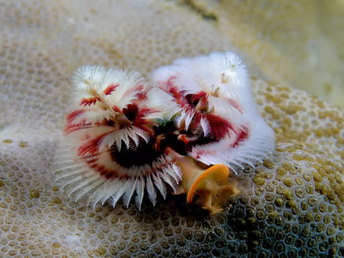
\includegraphics[width=\linewidth]{Resim1}
				\caption{\cite{ceylan2014hayvanlar}}
			\end{minipage}\hfill
			\begin{minipage}[t]{0.470\linewidth}
				\centering
				\includegraphics[width=\linewidth]{Resim2}
				\caption{\cite{ceylan2014hayvanlar}}
			\end{minipage}
			
			\vspace{0.5cm}
			
			\begin{minipage}[b]{0.470\linewidth}
				\centering
				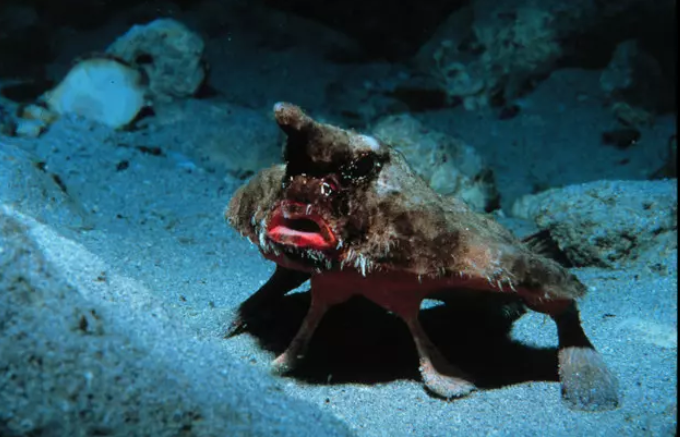
\includegraphics[width=\linewidth]{Resim3}
				\caption{\cite{ceylan2014hayvanlar}}
			\end{minipage}\hfill
			\begin{minipage}[b]{0.470\linewidth}
				\centering
				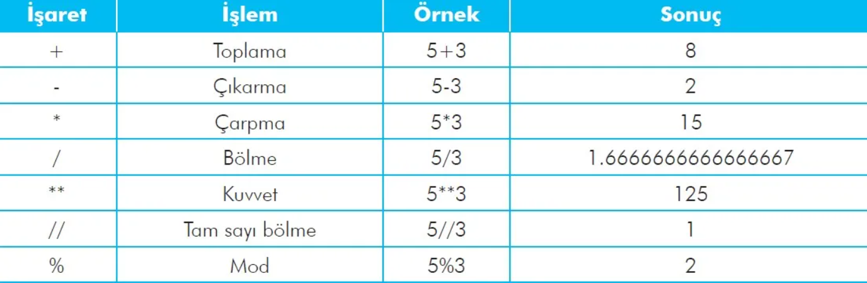
\includegraphics[width=\linewidth]{Resim4}
				\caption{\cite{stokfoto}}
			\end{minipage}
			
		\end{figure}
		
	\end{landscape}
	
	Zero-shot learning, bir modelin eğitim sırasında hiç görmediği sınıfları tanımayı veya bu sınıflara ait özellikleri öğrenmeyi amaçlayan bir makine öğrenimi yaklaşımıdır. Bu senaryoda, verilen bilgilere dayanarak "gavyal" resminin hangisi olduğunu tahmin etmeye çalışıyorsunuz.
	
	Verilen bilgiler:
	
	"Yakalanan en büyük gavyal 7 m. uzunluğunda idi, ama normalde uzunlukları 5 metreyi geçmez."
	"Balık yakalama yönünde evrimleşmiş uzun ve dar ağız yapısı"
	"Gavyal, tuzlu su timsahından sonra dünyanın en büyük timsah çeşididir."
	
	Bu bilgilere dayanarak, en büyük olasılıkla gavyal resminin 4. olduğunu söyleyebilirim. Çünkü 1. bilgi, diğerlerine göre daha spesifik bir özellik veriyor ve gavyalın uzunluğunun normalde 5 metreyi geçmeyeceğini belirtiyor. Dolayısıyla, bütün  resimler arasında seçim yaparken, bu bilgiyi göz önünde bulundurarak 4. resmin gavyal olma olasılığının daha yüksek olduğunu düşünüyorum. Bu nedenle, gavyal resminin 4. olduğunu tahmin ederdim.
	
	\clearpage
	
	\section* {5 Geliştirilmiş Blok Bazında Sınıflandırma}
	Geleneksel yöntemler blok bazlı regresyona dayanmaktadır. Ancak, bu Geliştirilmiş Blok Bazında Sınıflandırma (Enhanced Blockwise Classification (EBC)) çerçevesi, her blok içindeki sayı değerini birkaç önceden tanımlanmış aralığa sınıflandırmayı amaçlayan bir fikre dayanmaktadır. Geliştirme, üç ana noktadan gelmektedir: ayrıklaştırma politikası, etiket düzeltme ve kayıp fonksiyonu\cite{idrees2018composition}.
	\newline  
	
	
	 Bu yöntem, görüntüyü küçük bloklara böler ve her bir bloktaki nesne sayısını belirli bir aralığa sınıflandırmayı amaçlar. Bu sınıflandırma, belirli bir blok içindeki nesne sayısını tahmin etmeye odaklanır ve nesnelerin yoğunluğunu ölçmek için kullanılır.
	 \newline   
	 
	 
	  Ayrıklaştırma Politikası: EBC'de kullanılan ayrıklaştırma politikası, nesne sayısını belirli aralıklara sınıflandırmak için belirlenen stratejiyi ifade eder. Bu strateji, nesnelerin dağılımını en iyi şekilde yansıtmak için dikkatlice seçilir.
	 
	 Etiket Düzeltme: EBC, doğru etiketleme için bir düzeltme mekanizması içerir. Bu mekanizma, modelin öğrenirken daha doğru sonuçlar elde etmesine yardımcı olur ve modelin performansını artırır.
	 
	 Kayıp Fonksiyonu: EBC'nin kayıp fonksiyonu, modelin eğitilirken hata miktarını belirlemek için kullanılır. Bu kayıp fonksiyonu, modelin en iyi sınıflandırma sonuçlarını üretmek için optimize edilir.
	 
	 Bu üç bileşen, EBC'nin geliştirilmiş performansını sağlar ve nesne sayımı gibi görevlerde daha etkili bir şekilde çalışmasını sağlar.
	 
	 	\begin{figure}[!ht]
	 	\subcaptionsetup{labelformat=empty}
	 	\raggedright
	 	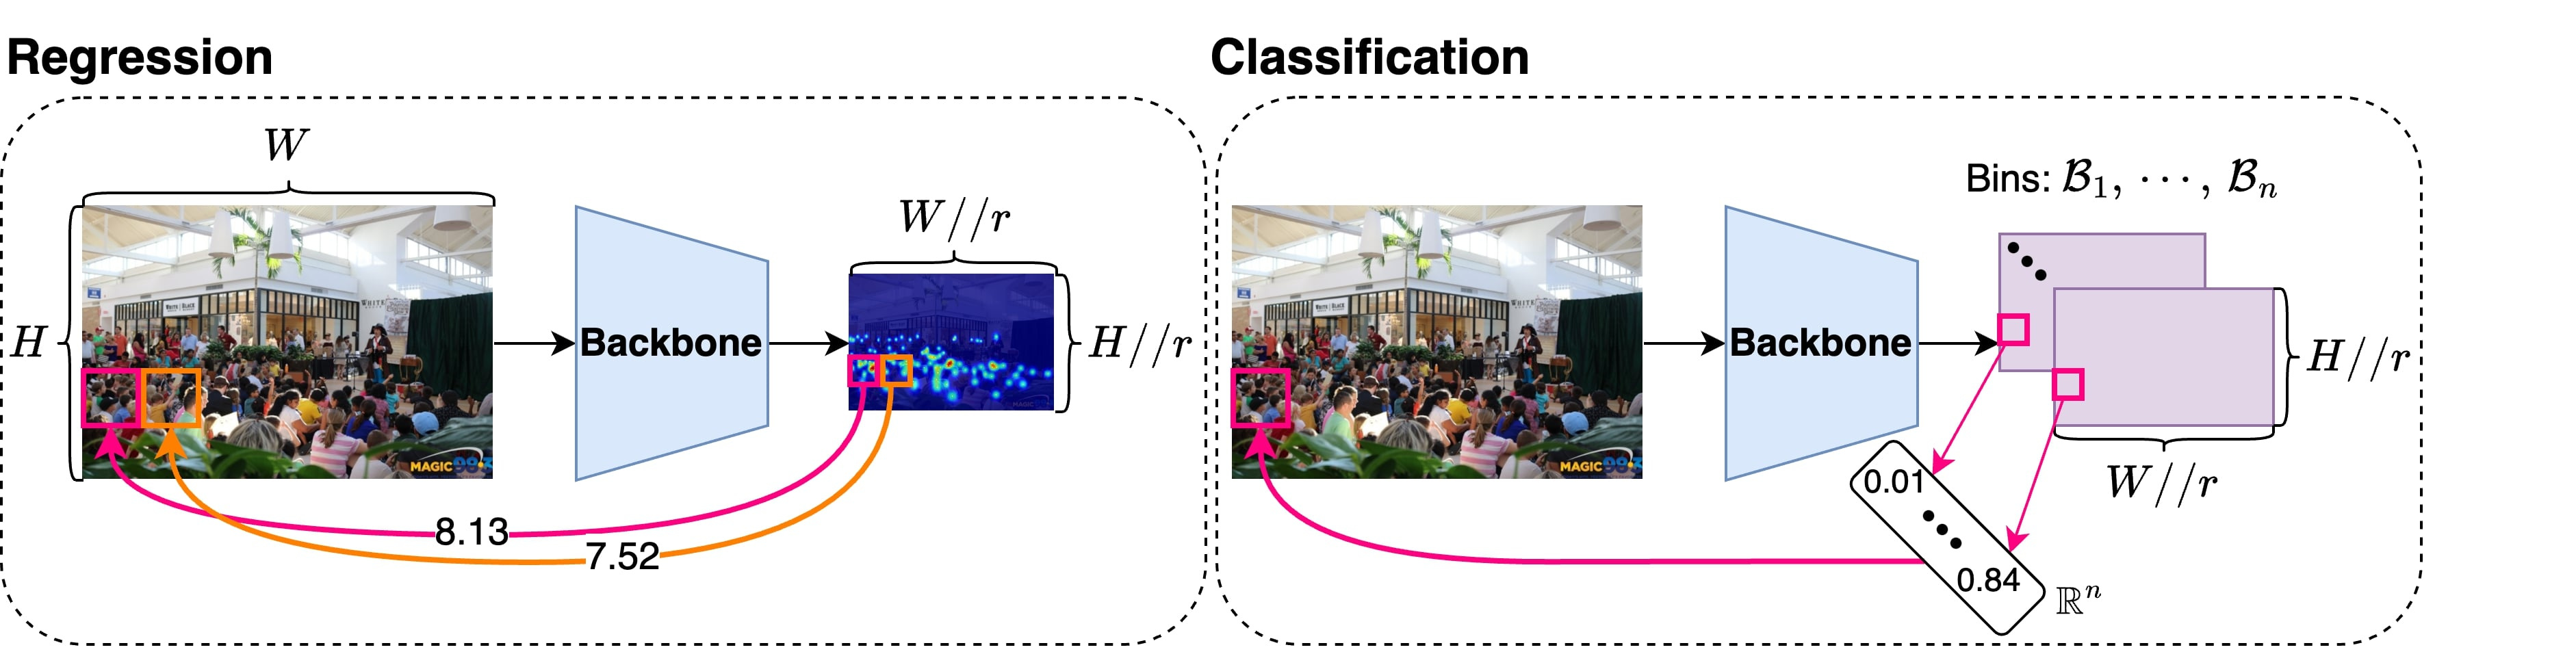
\includegraphics[width=\textwidth]{regression1}
	 	\caption{EBC \cite{idrees2018composition}}
	 	\label{Ornek_sonuc1}
	 \end{figure}

	 \begin{landscape} % Sayfayı döndürme
	 	
	 	\begin{figure}[p]
	 		\centering
	 		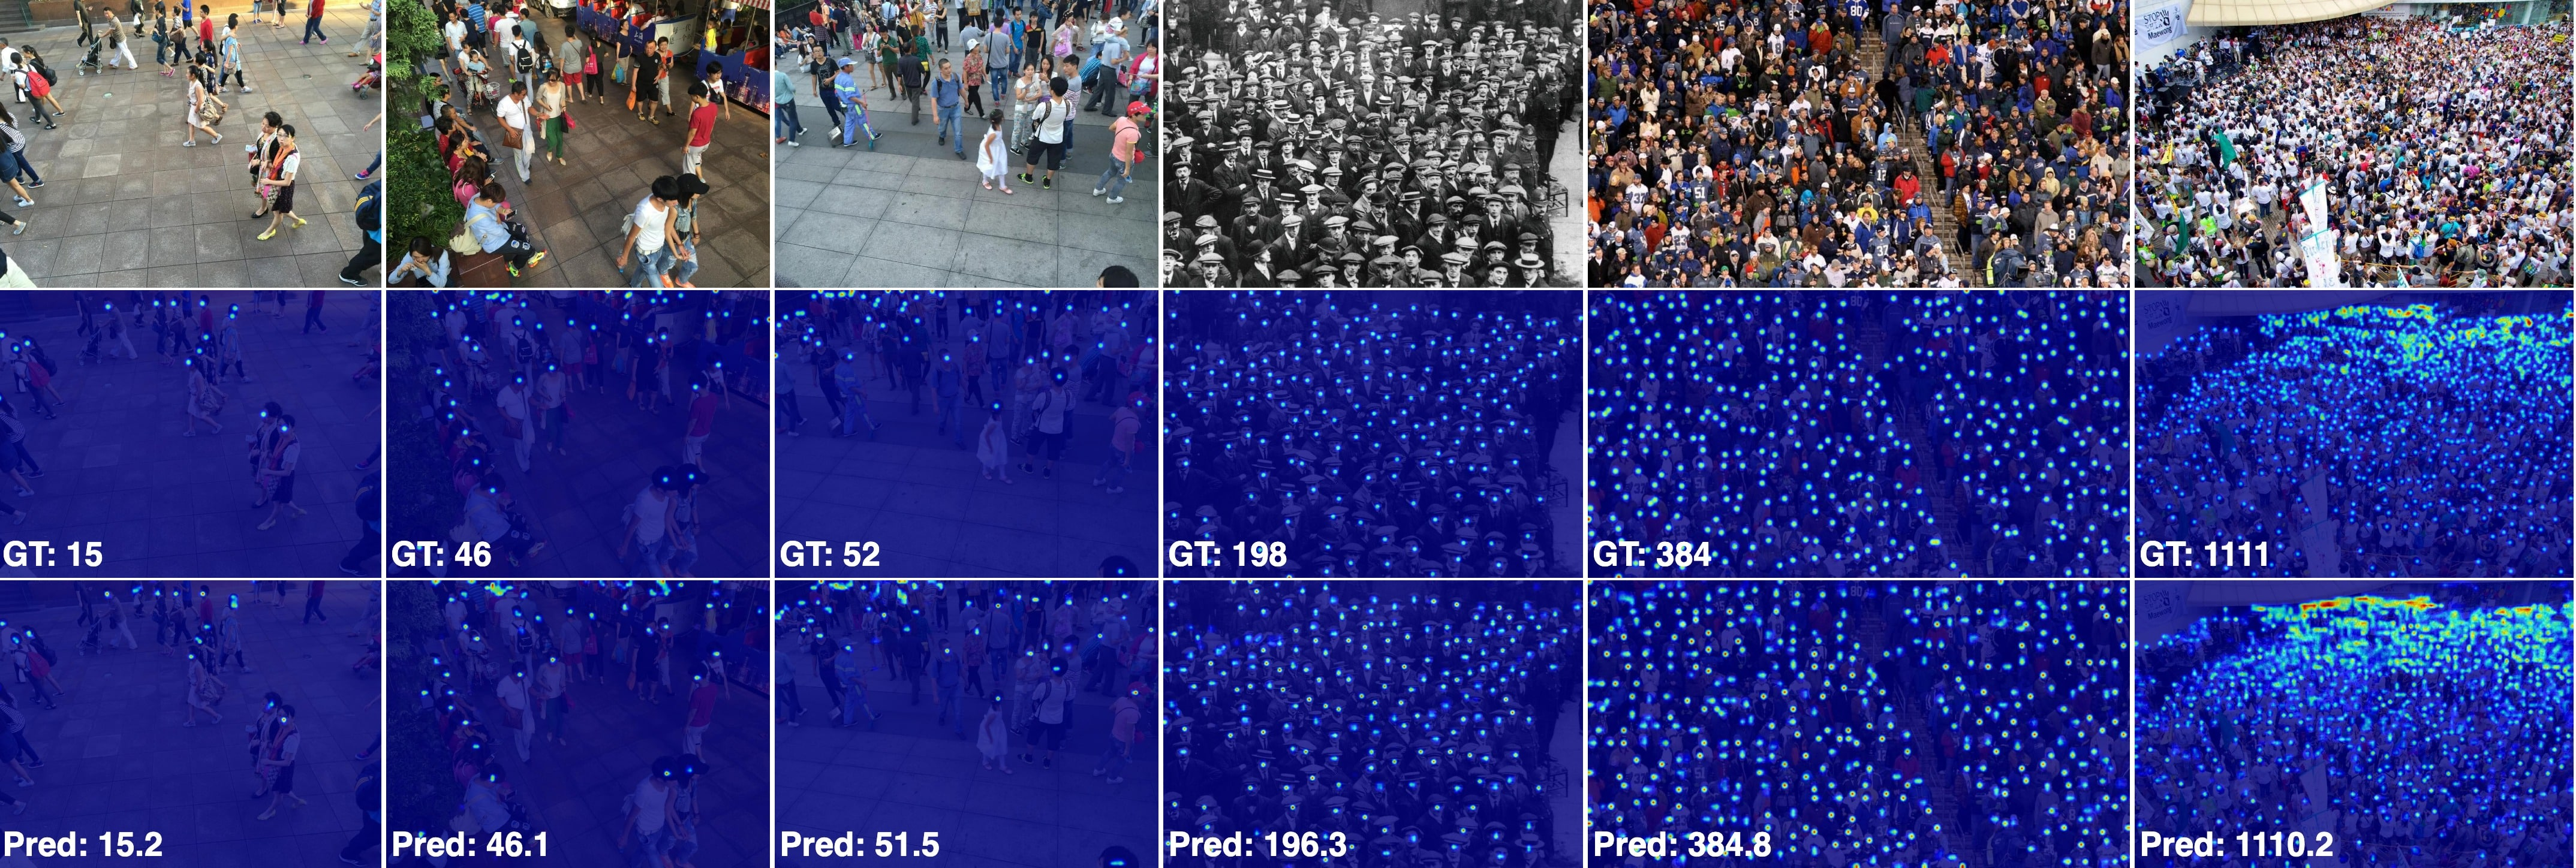
\includegraphics[width=\linewidth]{visualization}
	 		\caption{Proje Çıktısı Örneği \cite{ma2024clip} tarafından sağlanan görüntü.}
	 	\end{figure}
	 	
	 \end{landscape}
	 
	
	
	\clearpage
	

	
	
	\begin{figure}[!h]
		\section*{6 Dataset Örnekleri}
		Proje için incelenmiş birkaç veri setlerinin örnekleri aşağıdaki gibidir:
		
		\begin{subfigure}{\textwidth}
			\raggedright
			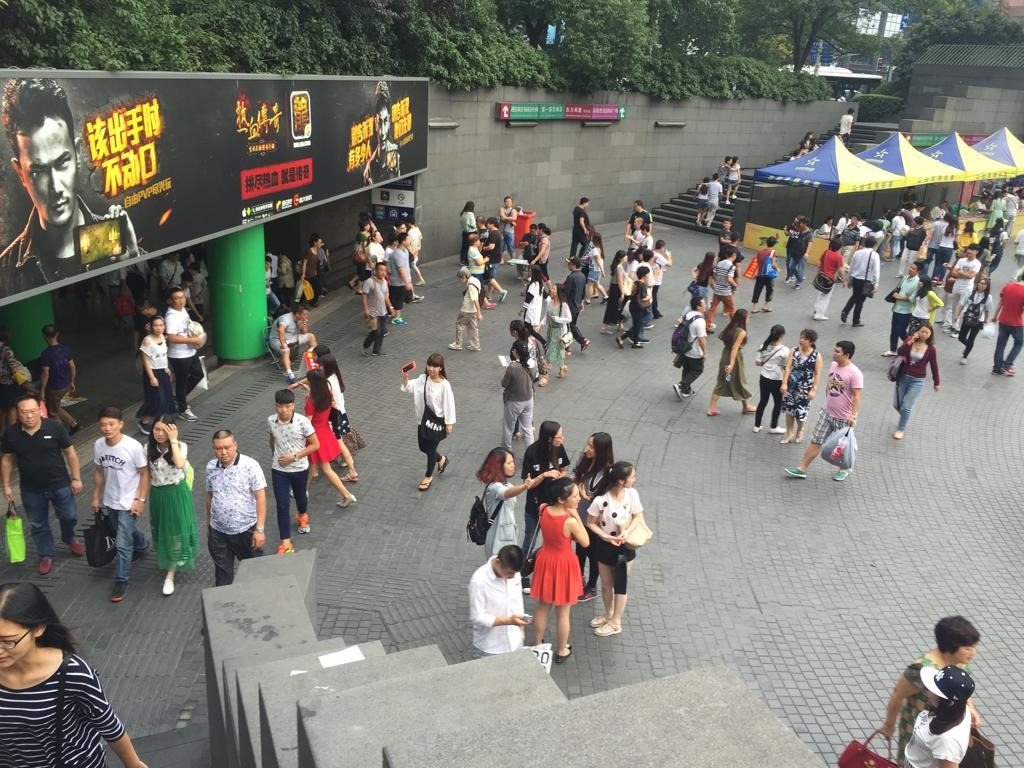
\includegraphics[width=\textwidth]{ornek1.jpg}
			\caption{Kalabalık Örnek Resmi 1 \cite{shanghaitechdataset} }
			\label{Ornek1}
		\end{subfigure}
		\begin{subfigure}{\textwidth}
			\raggedright
			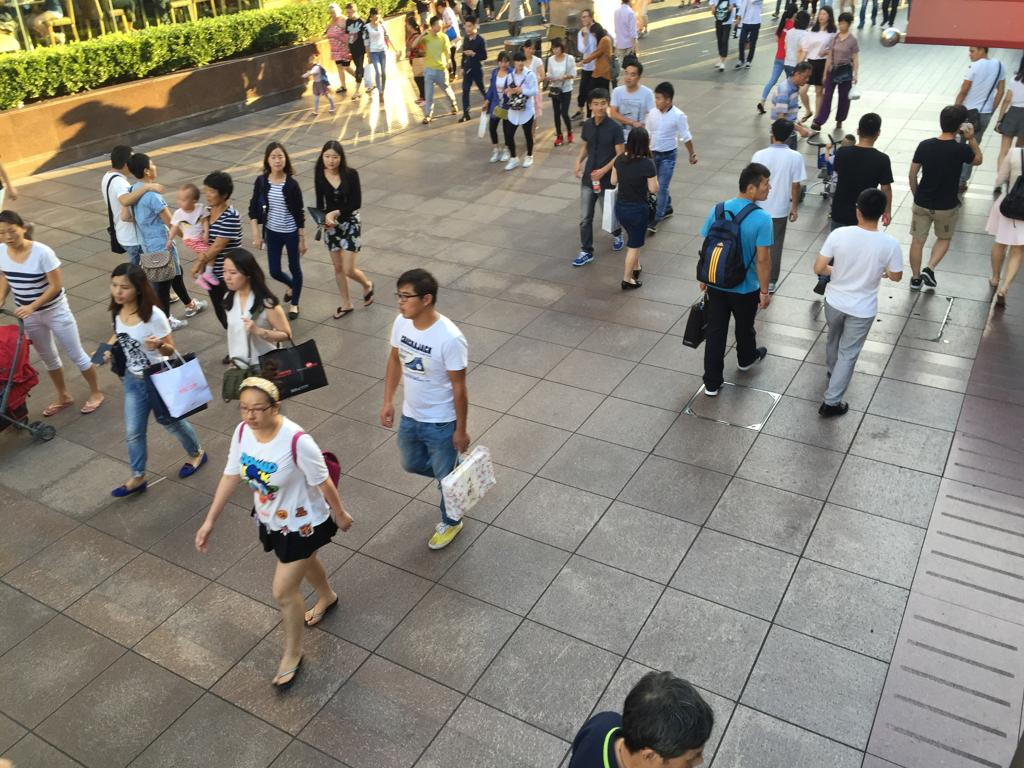
\includegraphics[width=\textwidth]{ornek2.jpg}
			\caption{Kalabalık Örnek Resmi 2 \cite{shanghaitechdataset}}
			\label{Ornek2}
		\end{subfigure}
	\end{figure}
	
	
	
	\begin{figure}[!h]
		\subcaptionsetup{labelformat=empty}
		\begin{subfigure}{\textwidth}
			\raggedright
			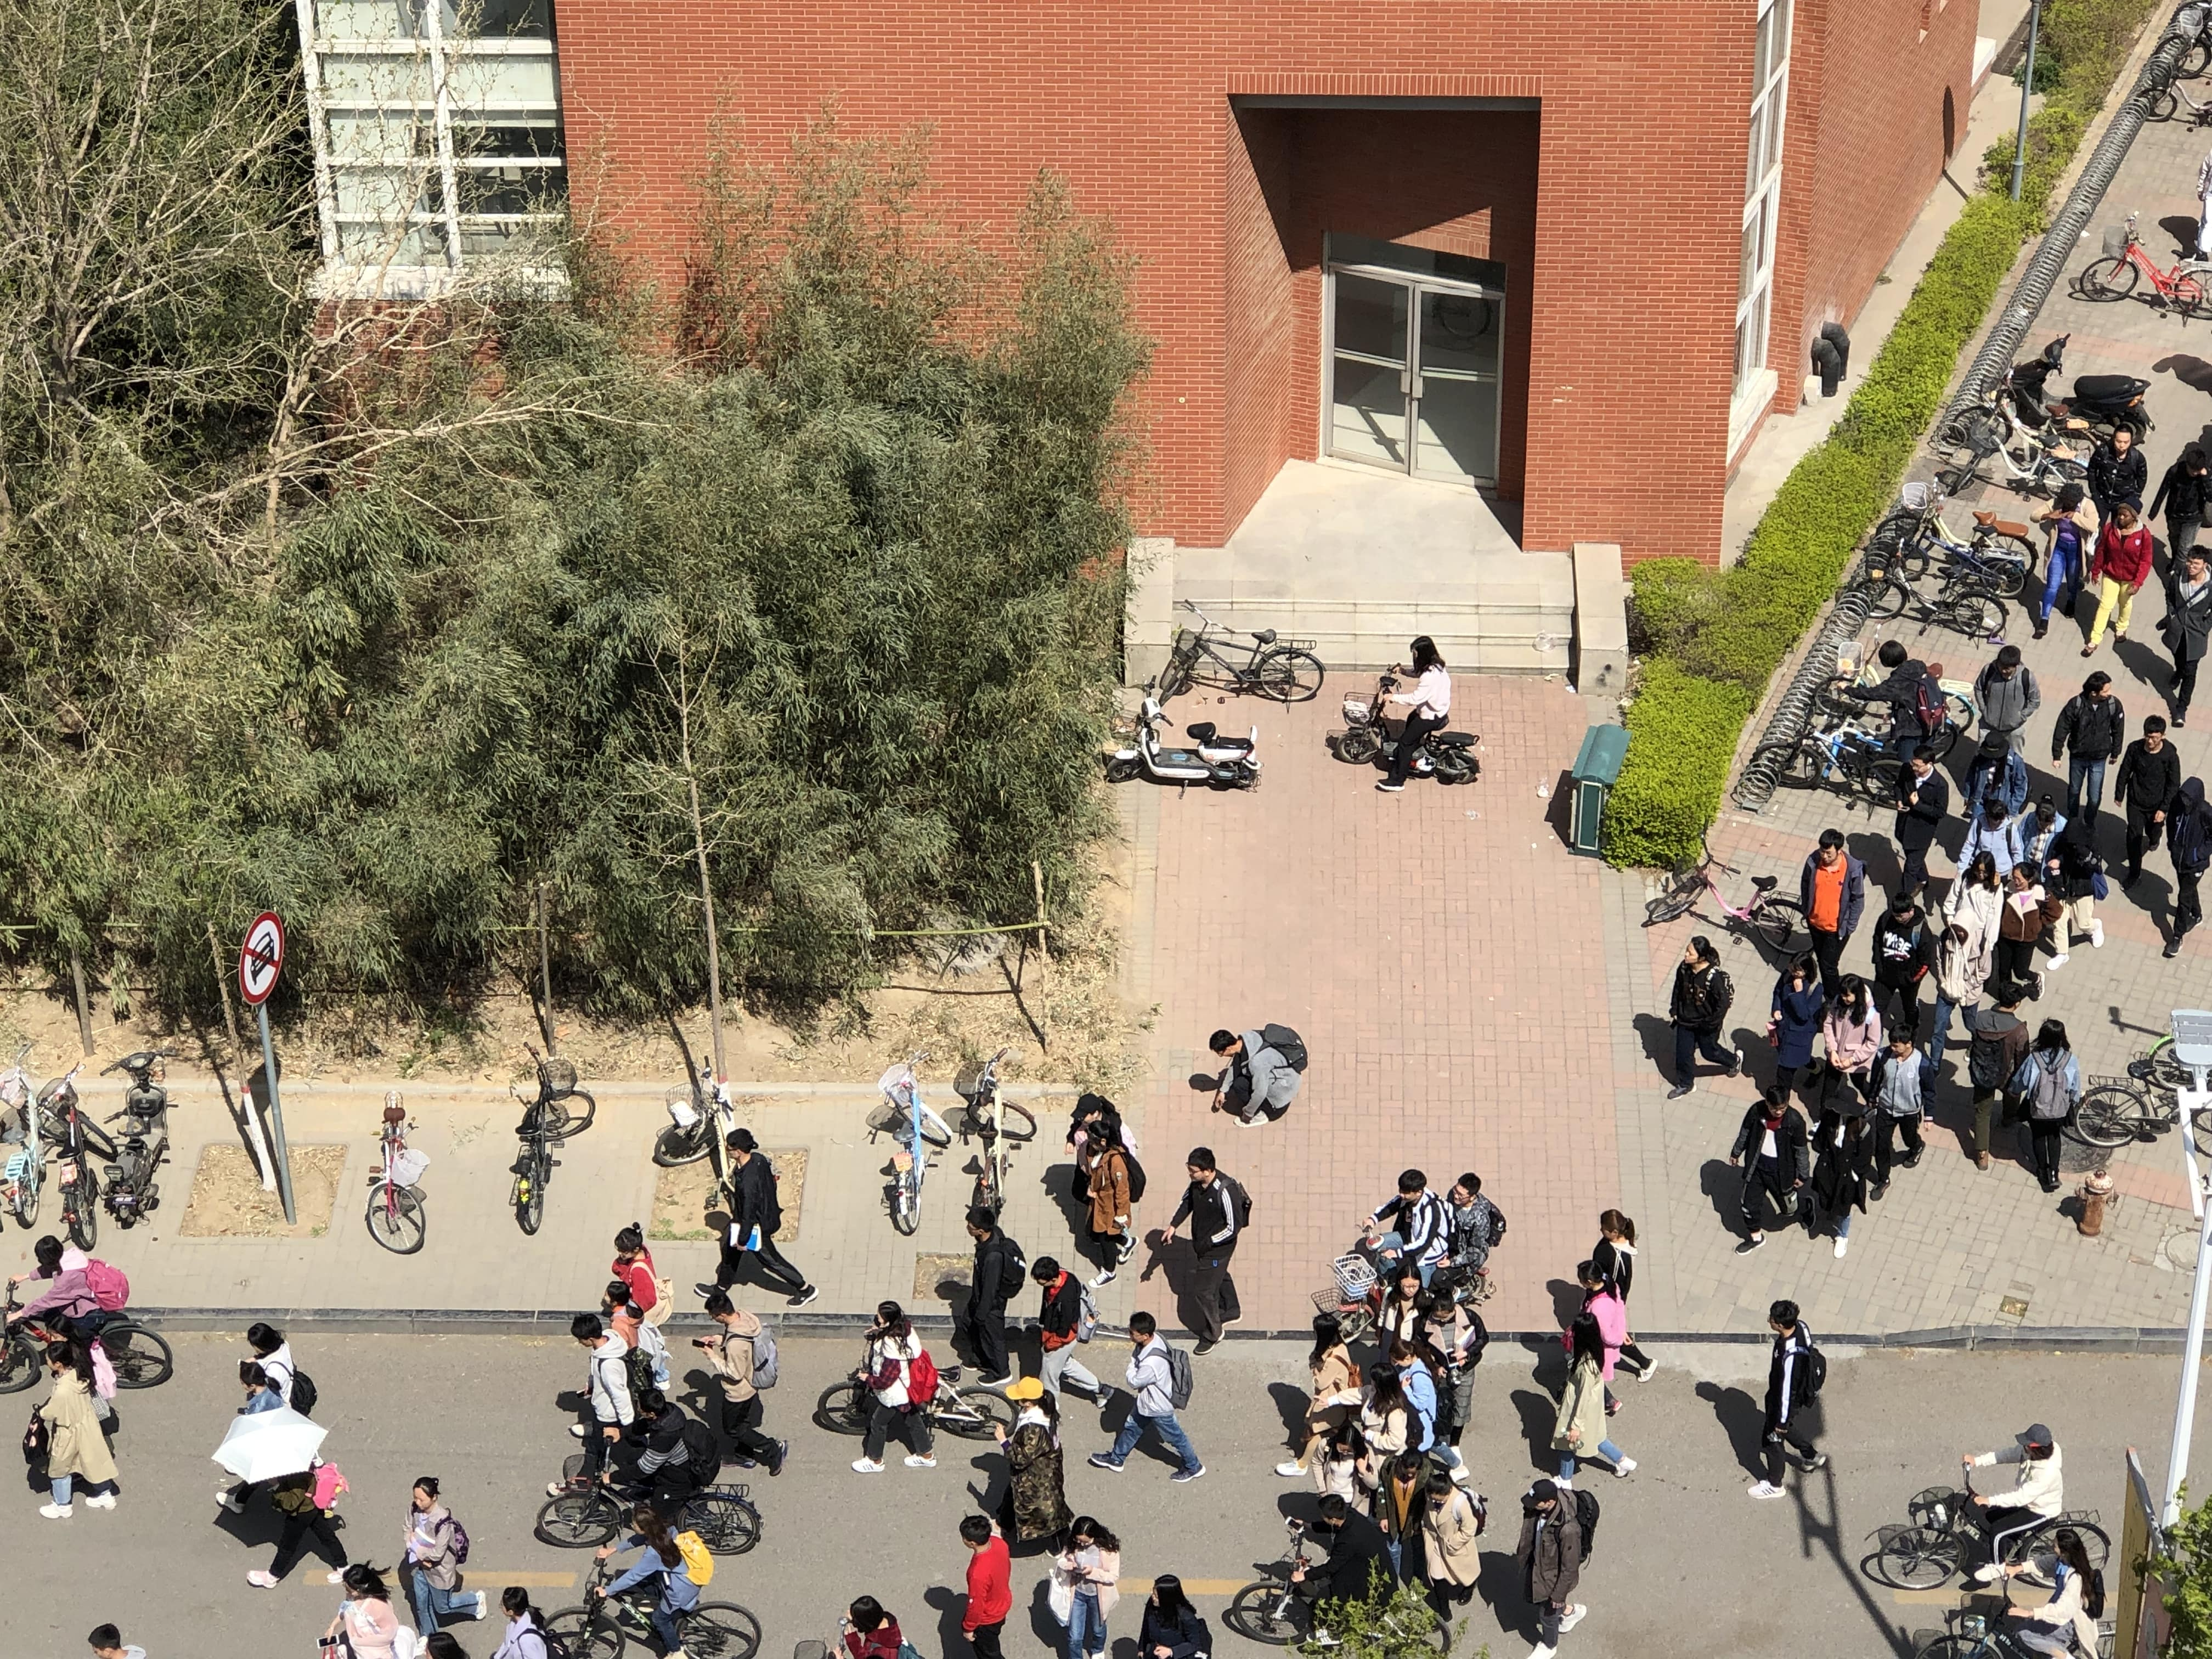
\includegraphics[width=\textwidth]{NPWU1}
			\caption{Kalabalık Örnek Resmi 3 \cite{wang2020nwpu}}
			\label{Ornek3}
		\end{subfigure}
		\begin{subfigure}{\textwidth}
			\raggedright
			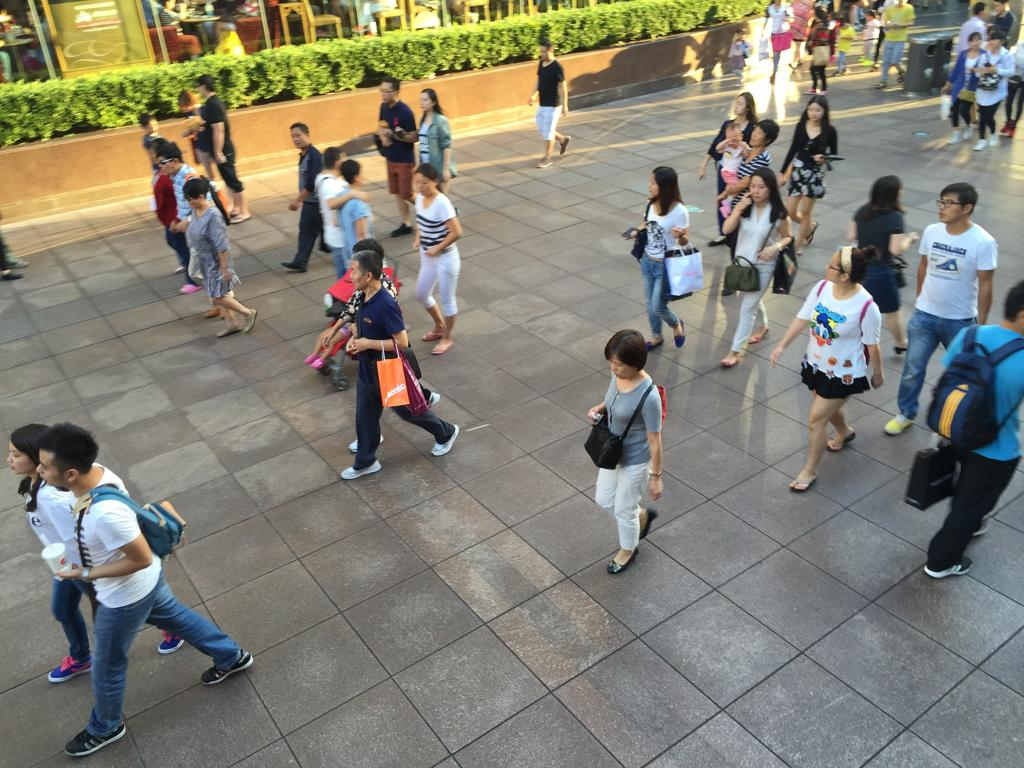
\includegraphics[width=\textwidth]{ornek4.jpg}
			\caption{Kalabalık Örnek Resmi Örnek 4 \cite{shanghaitechdataset}}
			\label{Ornek4}
		\end{subfigure}
	\end{figure}
	
	
	\begin{figure}[!h]
		\subcaptionsetup{labelformat=empty}
		\begin{subfigure}{\textwidth}
			\raggedright
			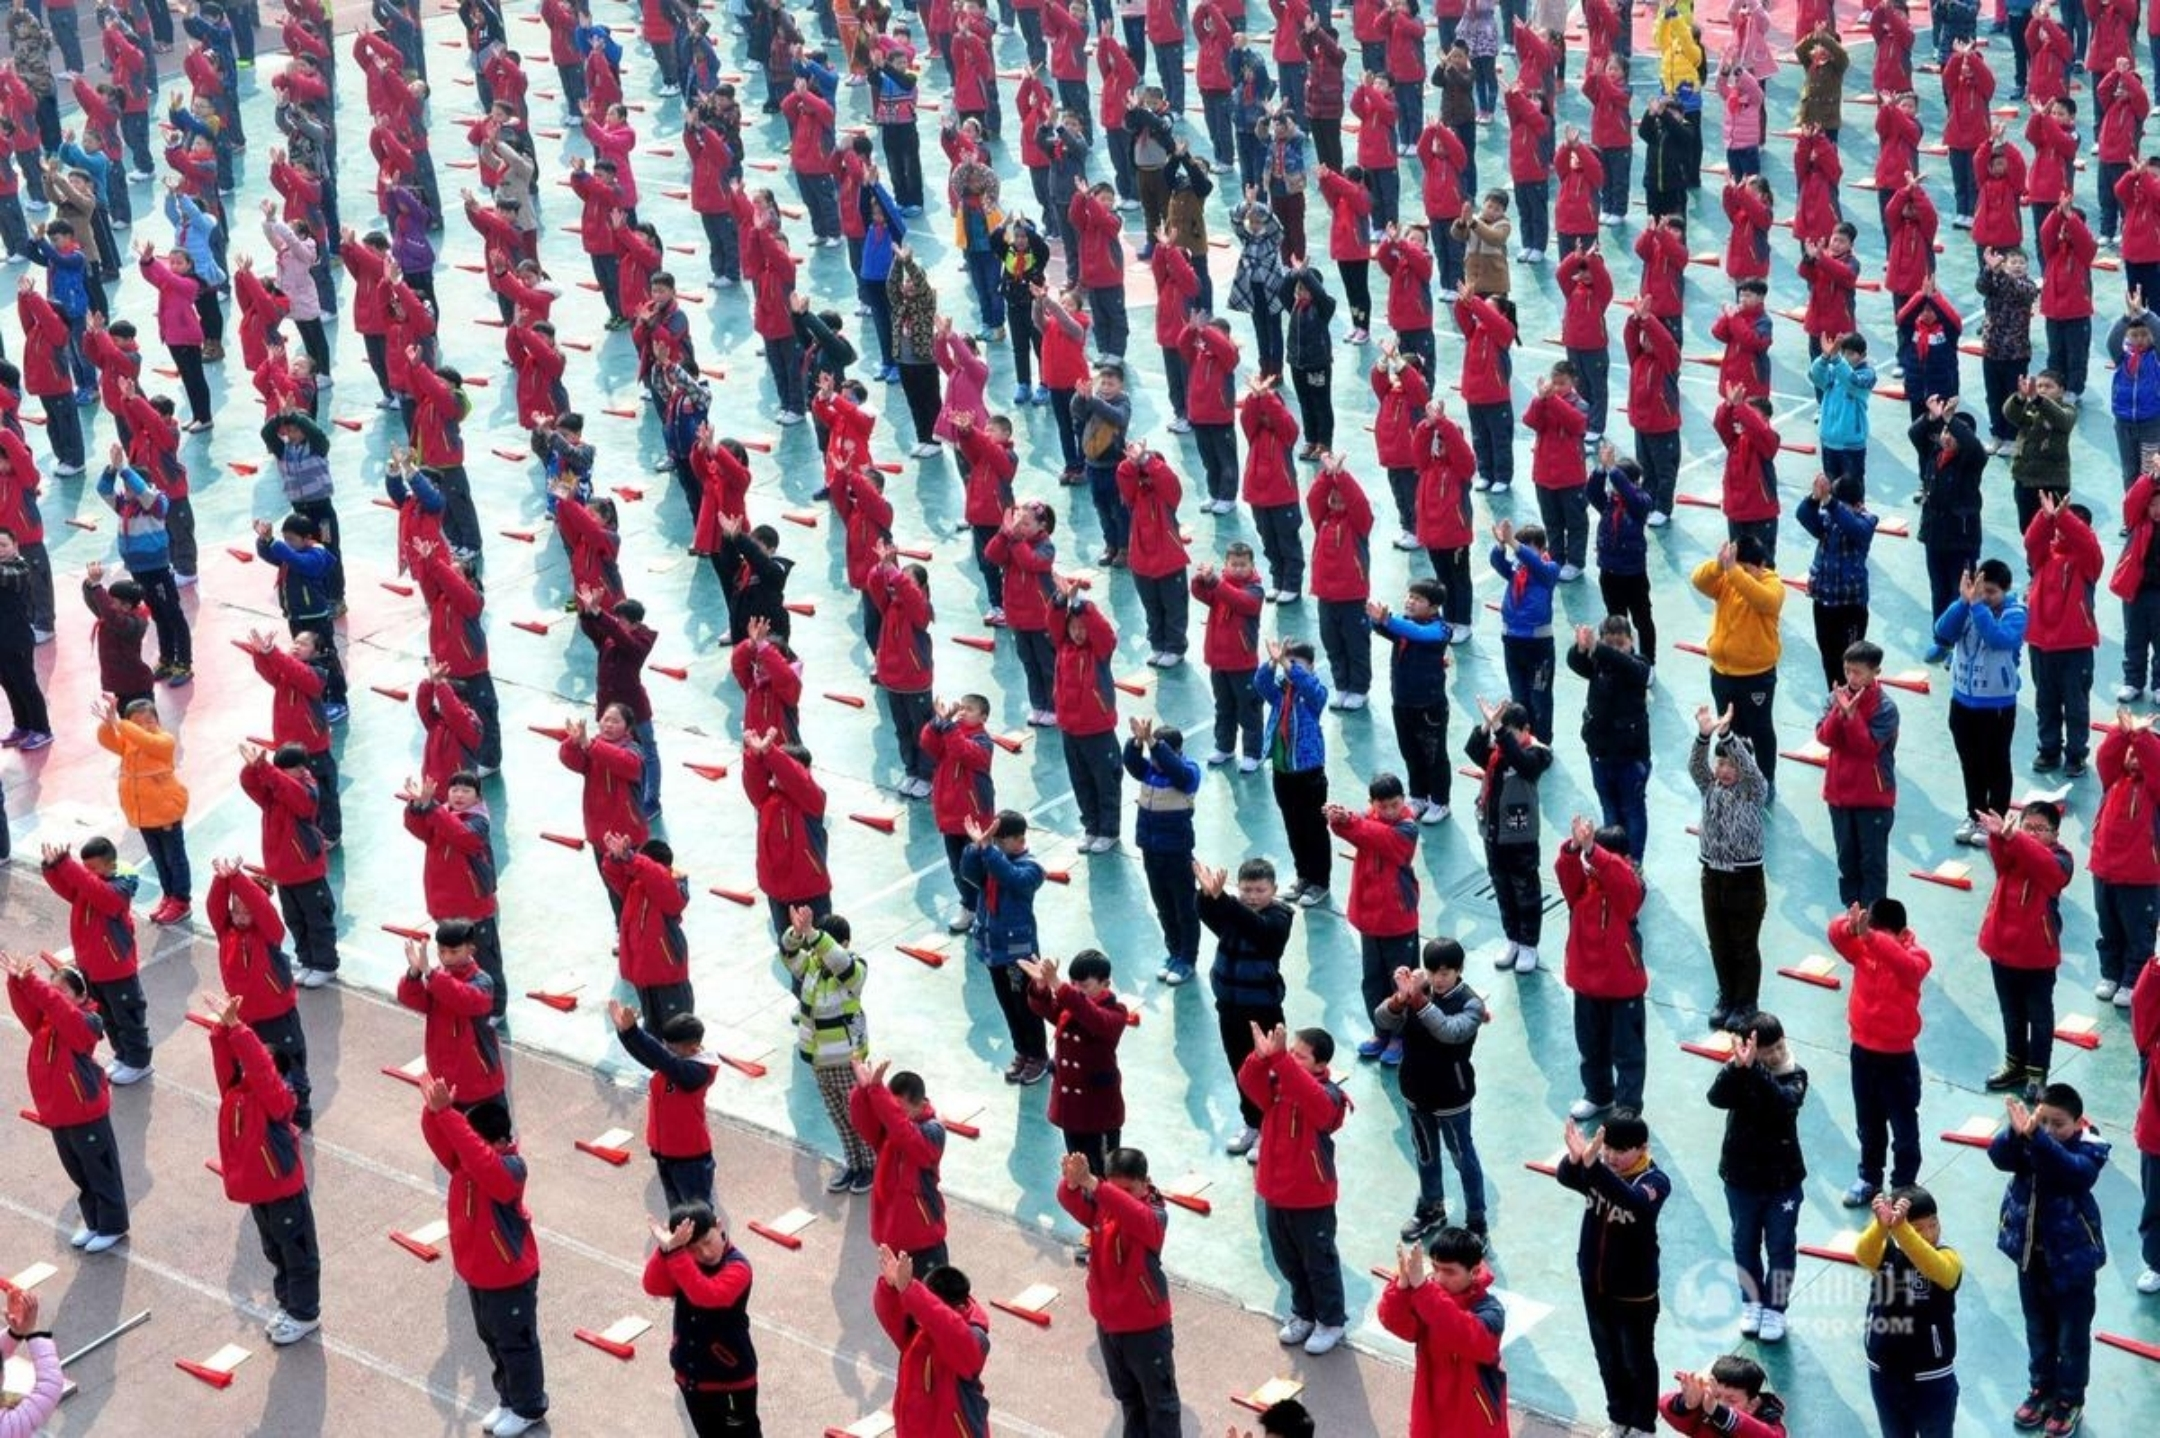
\includegraphics[width=\textwidth]{NPWU2}
			\caption{Kalabalık Örnek Resmi 5 \cite{wang2020nwpu}}
			\label{Ornek5}
		\end{subfigure}
		\begin{subfigure}{\textwidth}
			\raggedright
			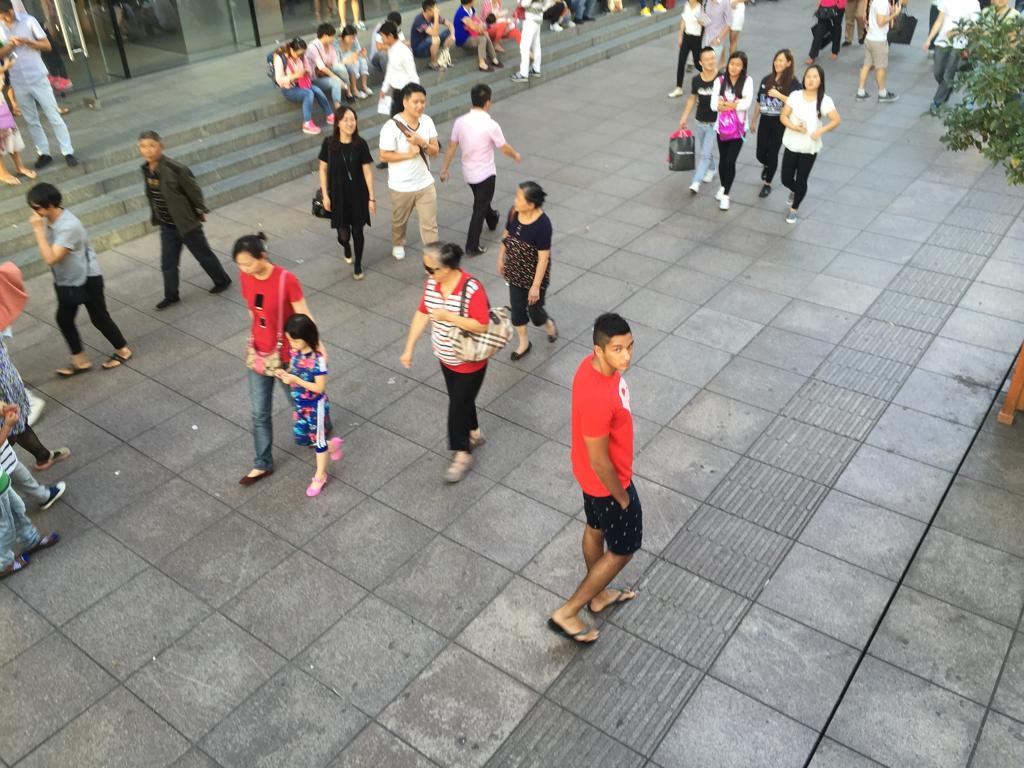
\includegraphics[width=\textwidth]{ornek6.jpg}
			\caption{Kalabalık Örnek Resmi 6 \cite{shanghaitechdataset}}
			\label{Ornek6}
		\end{subfigure}
	\end{figure}
	
	\begin{figure}[!h]
		
		\raggedright
		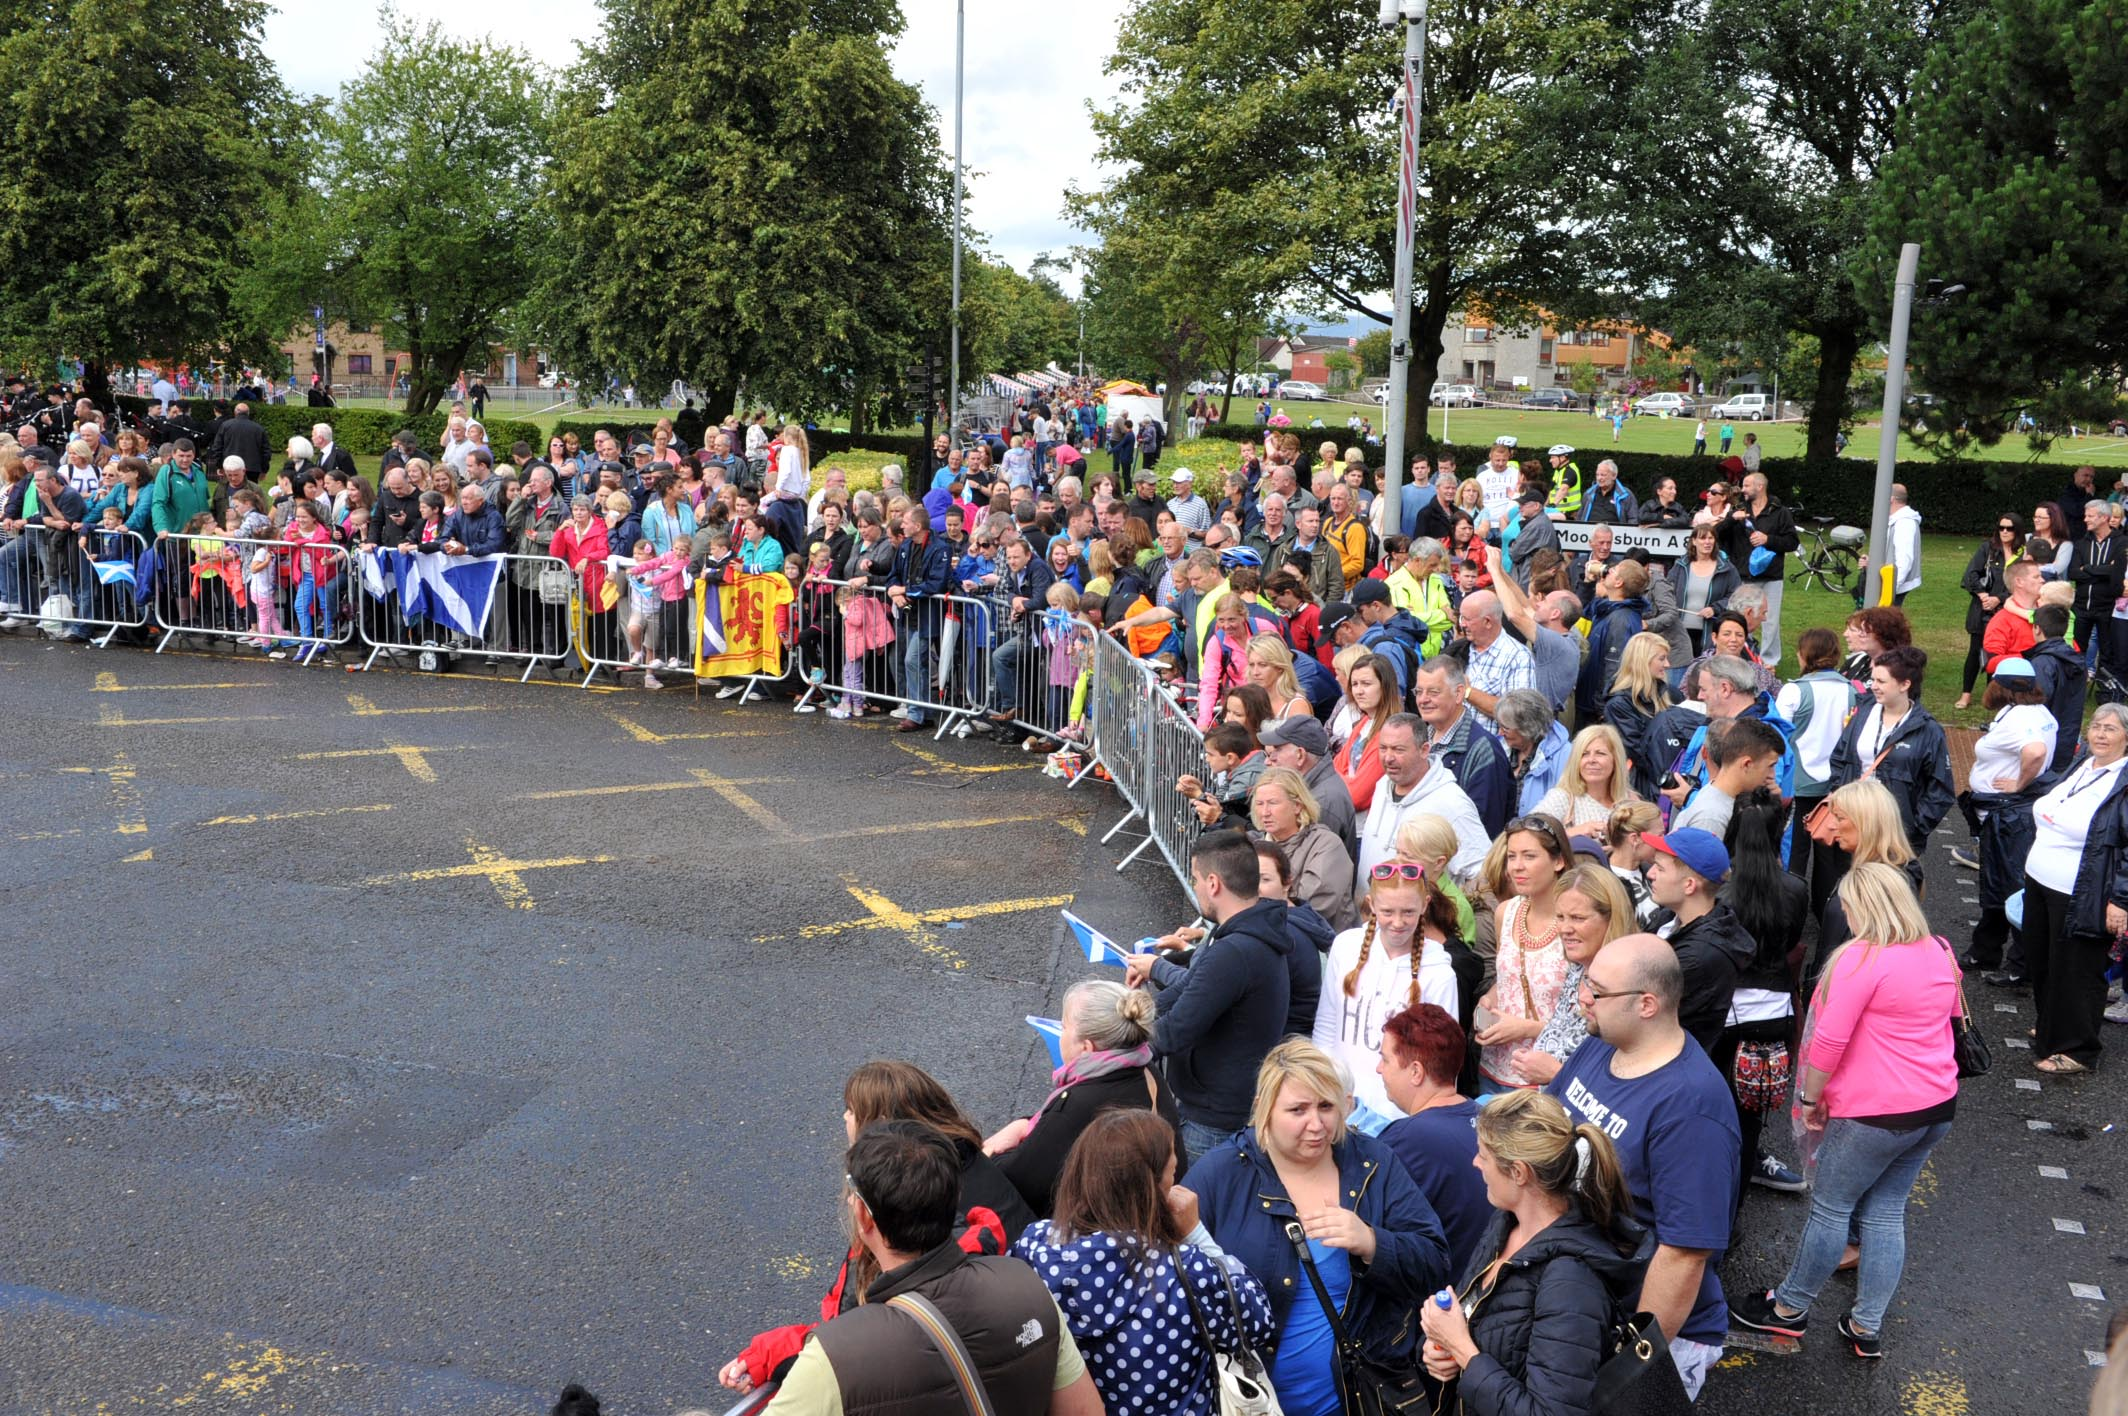
\includegraphics[width=\textwidth]{QNRF1}
		\caption{Kalabalık Örnek Resmi 7 \cite{2018composition2}}
		\label{Ornek_sonuc1}
	\end{figure}
	
	\begin{figure}[!h]
		
		\raggedright
		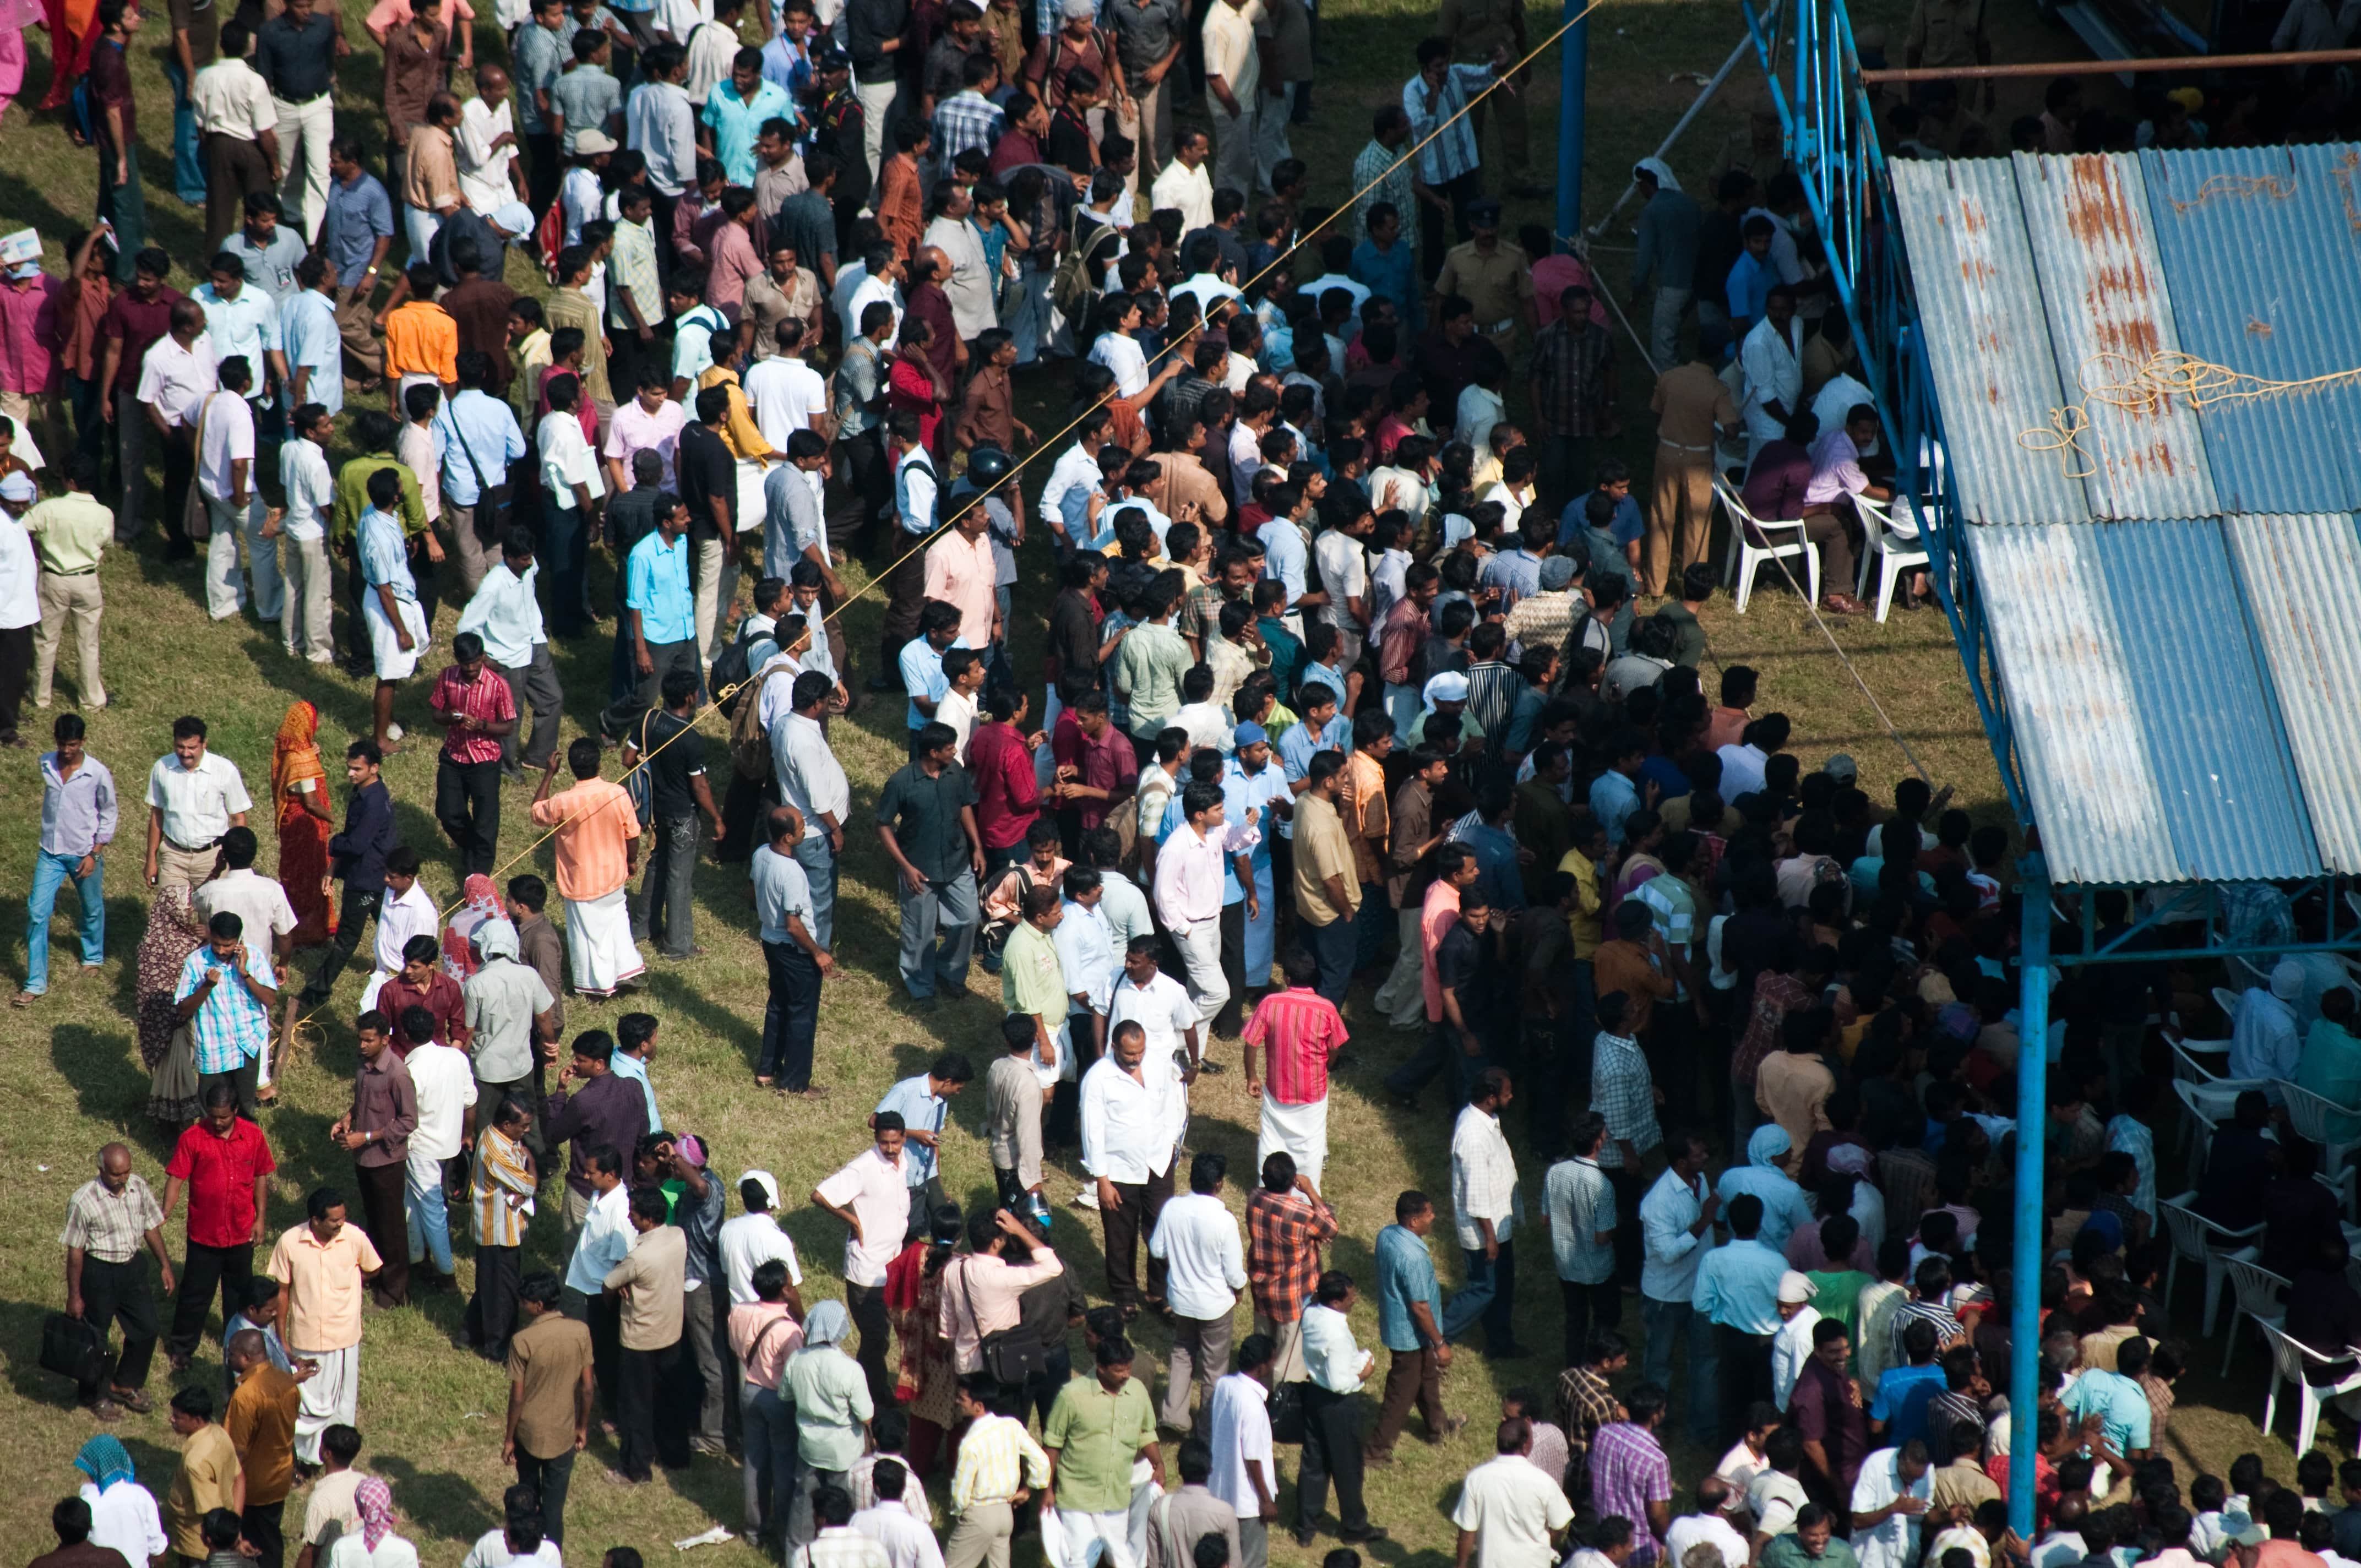
\includegraphics[width=\textwidth]{QNRF2}
		\caption{Kalabalık Örnek Resmi 8 \cite{2018composition2}}
		\label{Ornek_sonuc2}
	\end{figure}
	
		\begin{figure}[!h]
		\subcaptionsetup{labelformat=empty}
		\begin{subfigure}{\textwidth}
			\raggedright
			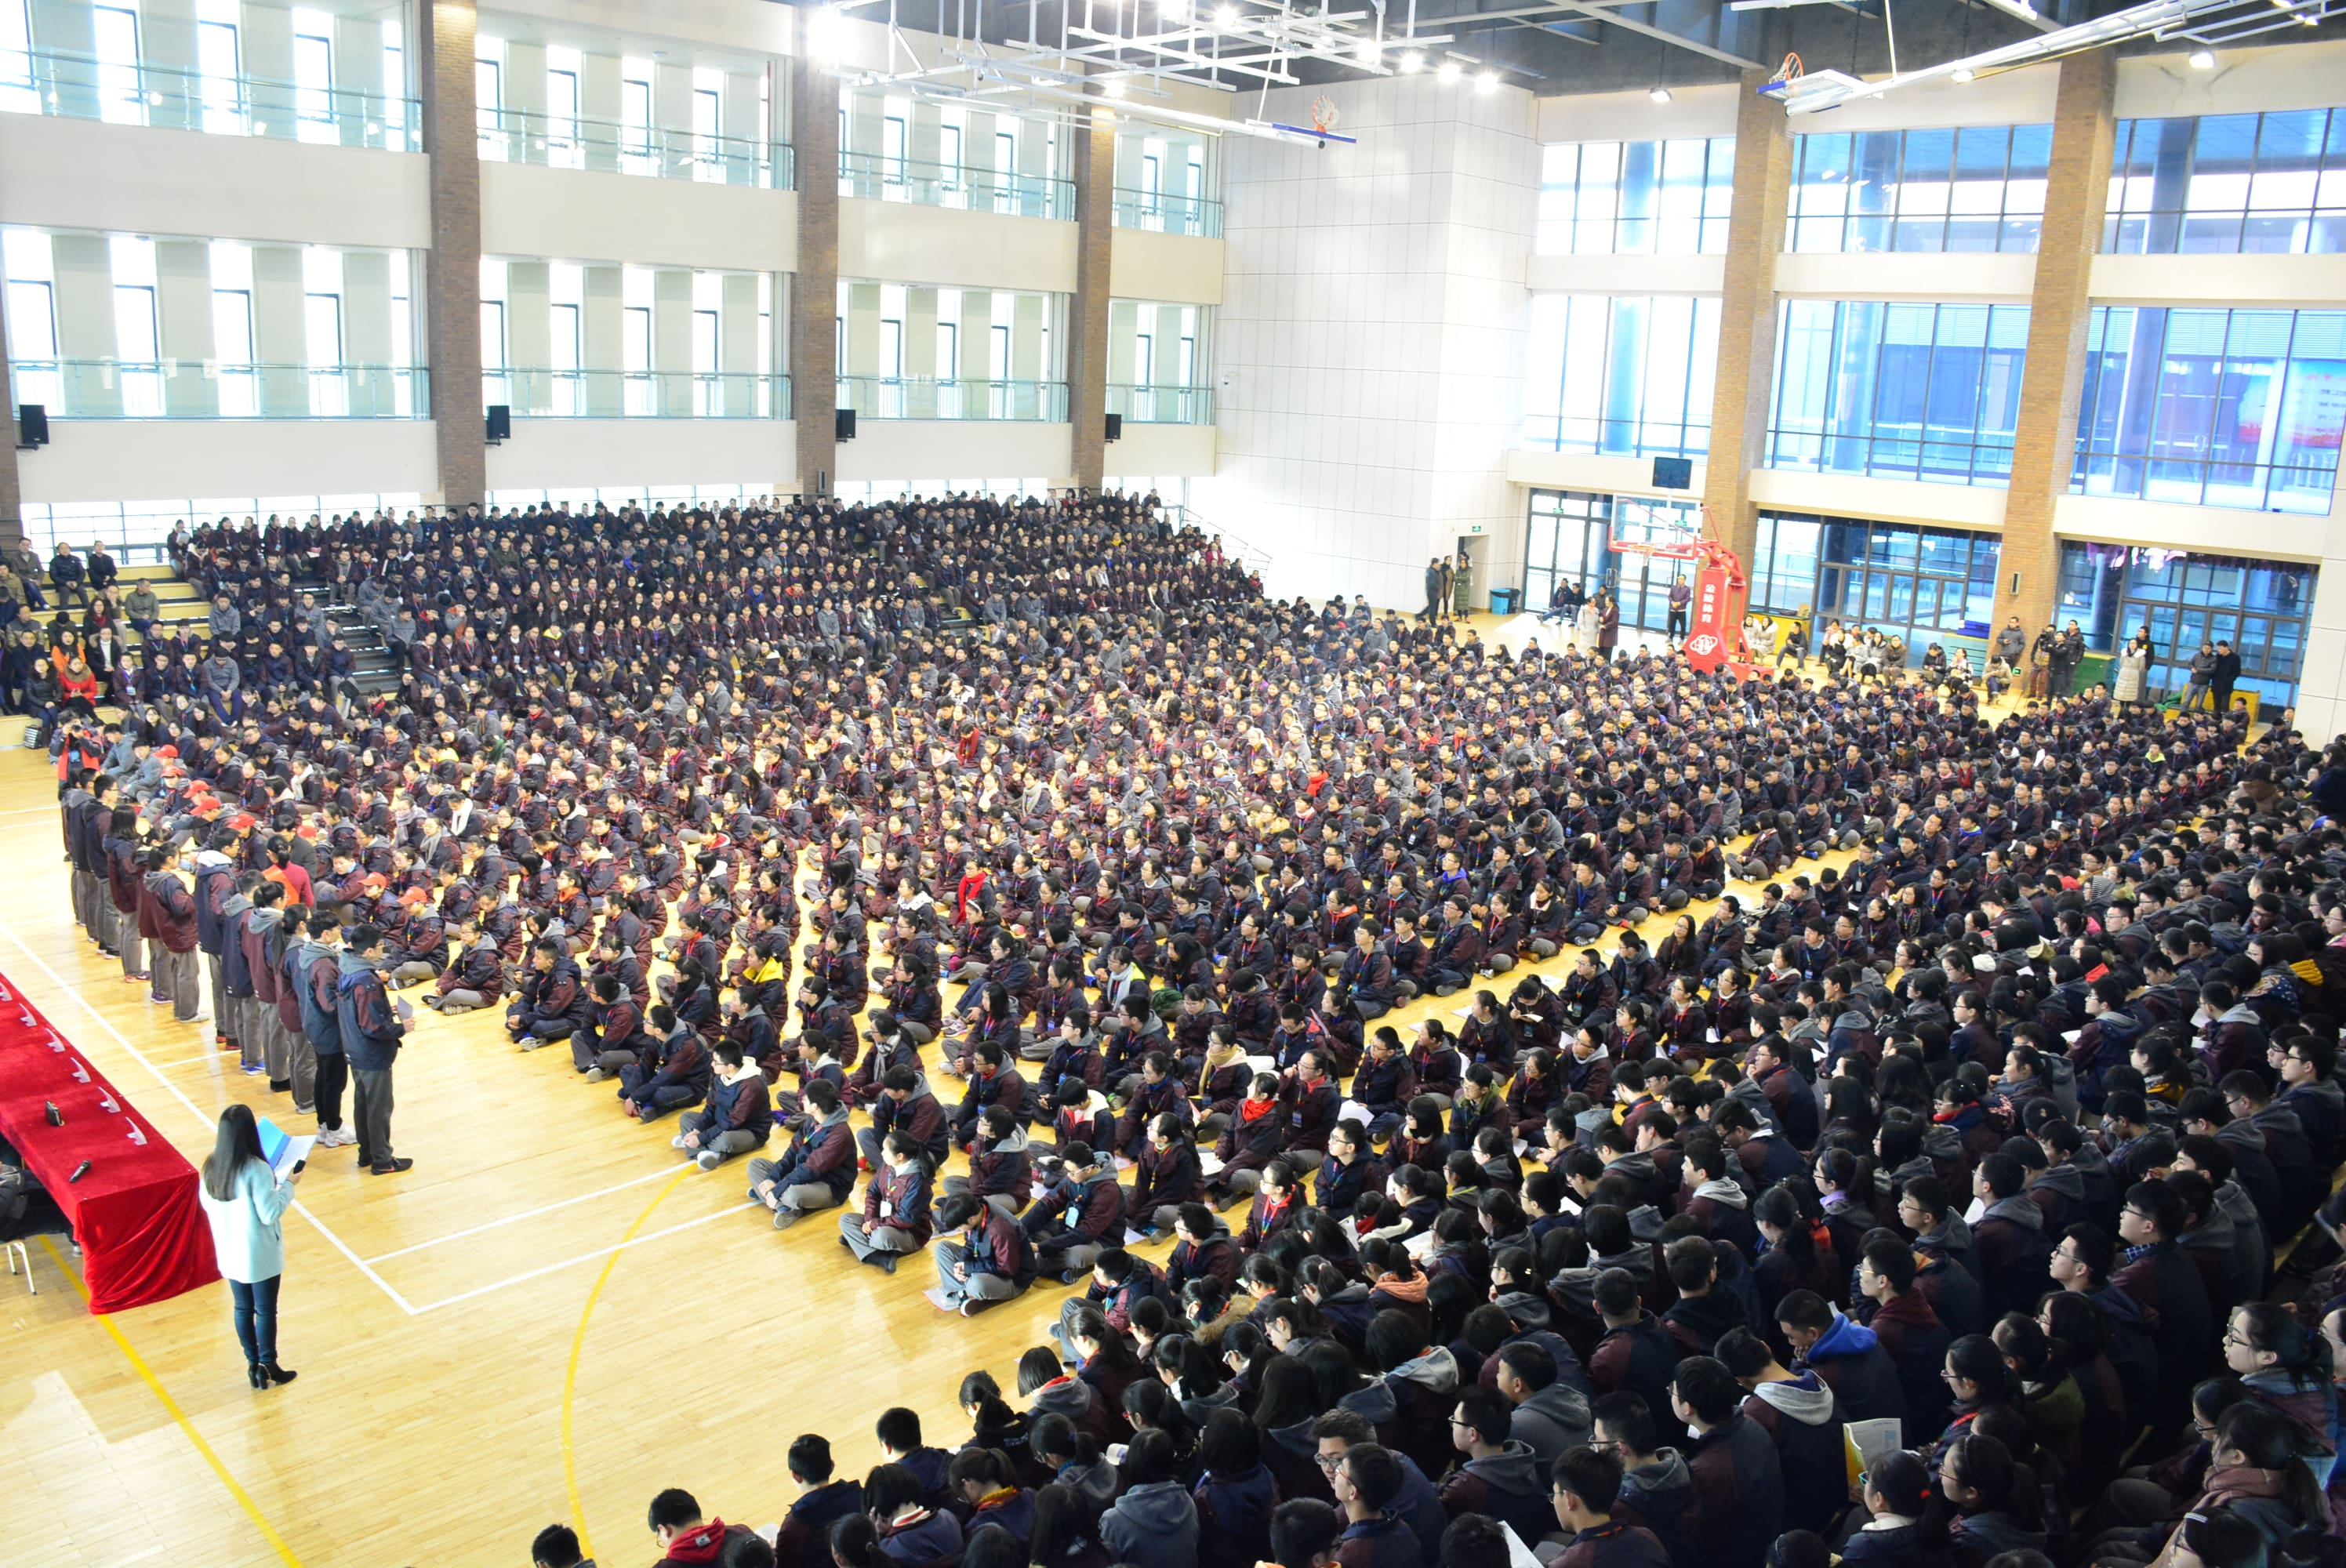
\includegraphics[width=\textwidth]{NPWU3}
			\caption{Kalabalık Örnek Resmi 9 \cite{wang2020nwpu}}
			\label{Ornek5}
		\end{subfigure}
		\begin{subfigure}{\textwidth}
			\raggedright
			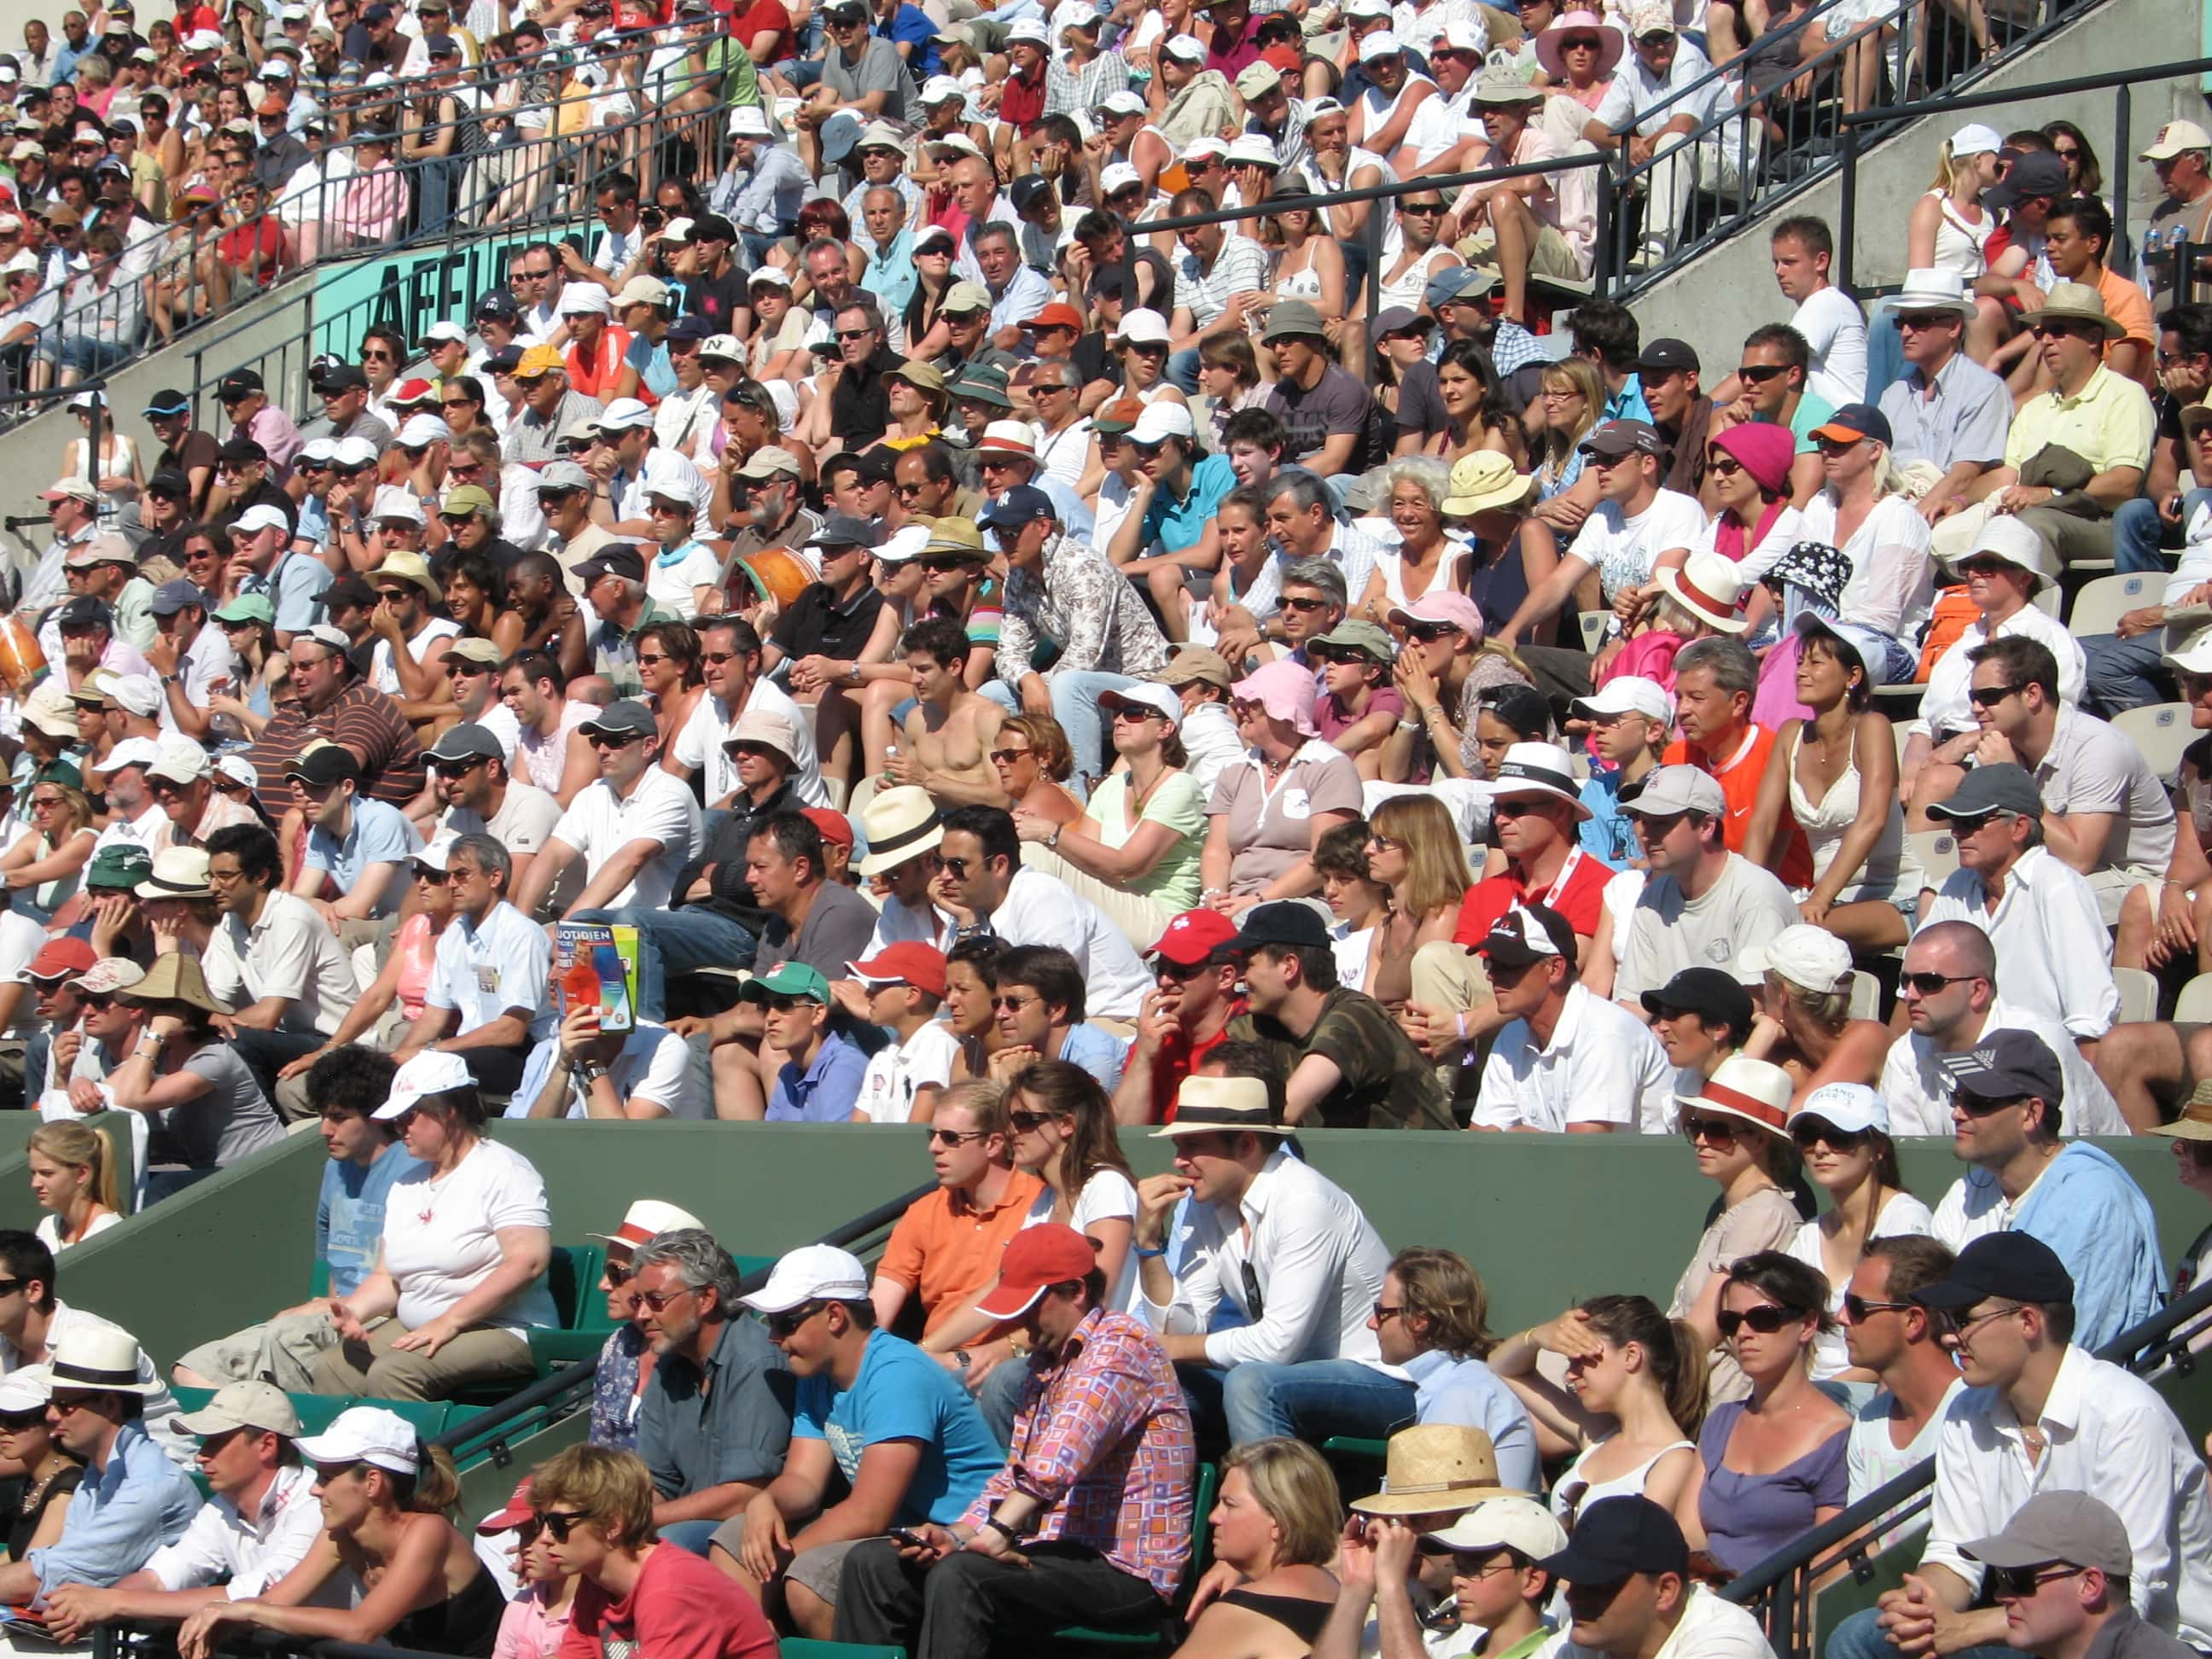
\includegraphics[width=\textwidth]{QNRF3}
			\caption{Kalabalık Örnek Resmi 10  \cite{2018composition2}}
			\label{Ornek6}
		\end{subfigure}
	\end{figure}
	

	
	
	\clearpage
	


	
	
	
	\section*{7 Alınan Hatalar}
	
	\begin{figure}[!h]
		
		\centering
		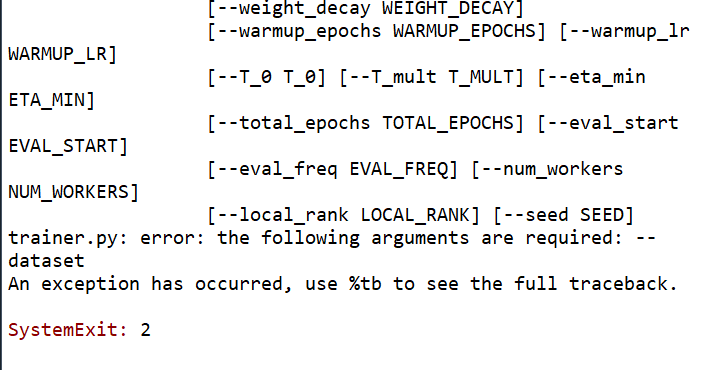
\includegraphics[width=\linewidth]{Hata1}
		\caption{\cite{ma2024clip}}
		
		
	\end{figure}
	\raggedright
	Bu talimatlar, bir Python betiğini veya modülünü Jupyter Notebook veya diğer not defteri uygulamalarında çalıştırırken karşılaşılan bir durumu ele alıyor. Örneğin, bir betik veya modül yazdınız ve bu kodu Jupyter Notebook'ta veya başka bir not defteri uygulamasında çalıştırmak istiyorsunuz.
	
	\begin{verbatim}
		required=True ifadesini  required=False\end{verbatim} olarak değiştirmek, betiğinizi esnek hale getirir. Artık argümanlar zorunlu değil, yani kullanıcılar bunları belirtmek zorunda değiller. Eğer belirtilmezse, kod varsayılan bir değer kullanır.
	
	\begin{verbatim}
		ap.add_argument("-f", gerekli=False)	\end{verbatim}
	
	ifadesi ise Jupyter Notebook veya diğer not defteri uygulamalarında argparse'ın özel bir durumunu ele alıyor. -f argümanı, Jupyter Notebook'un kendi ihtiyaçları için kullanılır ve eğer belirtilmezse, kod hata vermez.
	
	
	Bu değişiklikler, betiğinizi veya modülünüzü Jupyter Notebook veya diğer not defteri uygulamalarında daha rahat ve sorunsuz bir şekilde kullanmanızı sağlar. Kullanıcılar istediklerinde argümanları belirtebilirler, belirtmezlerse kod varsayılanları kullanır ve hata almazlar\cite{CB_Acnt}.
	
	\clearpage
	{\texttt{def standardize\_dataset\_name}}\texttt{(dataset: str) -> str:}
	\begin{verbatim}
		assert dataset.lower() in available_datasets, f"Dataset {dataset} is not available."
		if dataset.lower() in ["shanghaitech_a", "sha"]:
		return "sha"
		elif dataset.lower() in ["shanghaitech_b", "shb"]:
		return "shb"
		elif dataset.lower() in ["ucf_qnrf", "qnrf", "ucf-qnrf"]:
		return "qnrf"
		elif dataset.lower() in ["nwpu", "nwpu_crowd", "nwpu-crowd"]:
		return "nwpu"
		else: # dataset.lower() in ["jhu", "jhu_crowd", "jhu_crowd_v2"]
		return "jhu"
	\end{verbatim}
	
	Kod içeriğinde ilgili bölümlerdeki eksik dataset Hatası , dataset ismi verilerek düzeltildi.
	
	\texttt{ attempted relative import with no known parent package(çözülemedi)}
	\begin{verbatim}
		File c:\users\bakid\onedrive\belgeler\clip-ebc-main\datasets\crowd.py:11
		from .utils import get_id, generate_density_map
		
		ImportError: attempted relative import with no known parent package \newline
	\end{verbatim}
	
	Proje sahibi tarafından belirtilen gereksinimlere göre, ilgili kod bölümlerindeki eksiklikler tespit edilmiş ve gerekli düzeltmeler yapılmıştır
	
	
	
	
	
	\bibliographystyle{plain}
	\bibliography{references.bib} 
\end{document}